

\newpage

%----------------------------------------------------------------------------------------

\section{Road Network and Prices Drivers}{Transport Routier et Déterminants des Coûts}

\label{sec:energyprice}

Les interactions entre réseaux et territoires peuvent se manifester indirectement au sein de propriétés économiques locales de territoires : ainsi, le prix de l'énergie conditionne fortement l'impédance d'un réseau routier, et donc son impact sur les territoires, et réciproquement ce prix est localement produit par des sous-marchés qui sont partie intégrante des territoires. La géographie des prix du carburant est donc un marqueur indirect des interactions. Par exemple, \cite{orfeuil2012grand} (p.~307) suggère un lien entre prix de l'essence et crise immobilière en région parisienne.


\bpar{
The geography of fuel prices has many various implications, from its significant impact on accessibility to being an indicator of territorial equity and transportation policy. In this paper, we study the spatio-temporal patterns of fuel price in the US at a very high resolution using a newly constructed dataset collecting daily oil prices for two months, on a significant proportion of US gas facilities. These data have been collected using a specifically-designed large scale data crawling technology that we describe.
}{
La géographie des prix du carburant a de nombreuses applications variées, de son impact significatif sur l'accessibilité à son rôle comme indicateur d'équité territoriale et de politique de transports. Dans cette section, nous étudions les variations spatio-temporelles des prix du carburant aux Etats-Unis à une résolution très fine, par l'utilisation d'un nouveau jeu de données, donnant les prix journaliers sur deux mois pour une proportion significative des stations essence. Les données ont été collectées par l'intermédiaire d'une technologie de crawling à grande échelle élaborée spécifiquement, que l'on décrira.
}

\bpar{
We study the influence of socio-economic variables, by using complementary methods: Geographically Weighted Regression to take into account spatial non-stationarity, and linear econometric modeling to condition at the state and test county level characteristics. The former yields an optimal spatial range roughly corresponding to stationarity scale, and significant influence of variables such as median income or wage per job, with a non-simple spatial behavior that confirms the importance of geographical particularities. On the other hand, multi-level modeling reveals a strong state fixed effect, while county specific characteristics still have significant impact. Through the combination of such methods, we unveil the superposition of a governance process with a local socio-economical spatial process. We discuss one important application that is the elaboration of locally parametrized car-regulation policies.
}{
Nous étudions l'influence de variables socio-économiques, en utilisant des méthodes complémentaires : la Régression Géographique Pondérée pour tenir compte de la non-stationnarité spatiale, et une modélisation économétrique linéaire pour conditionner à l'Etat et tester des caractéristiques au niveau du Conté. La première fournit une portée spatiale optimale qui correspond globalement à l'échelle de stationnarité, et une influence significative des variables comme le revenu moyen ou le salaire par travail, avec un comportement spatial dont la non simplicité confirme l'importance des particularités géographiques. D'autre part, la modélisation multi-niveaux révèle un très fort effet Etat, alors que les caractéristiques spécifiques au Comté gardent un impact significatif. A travers la combinaison de ces méthodes, nous démontrons la superposition d'un processus de gouvernance avec un processus spatial socio-économique local. Nous discutons une application potentielle importante qui est l'élaboration de politiques de régulation automobiles localement paramétrisées.
}




%%%%%%%%%%%%%%%%%%%%%%
\subsection{Context}{Contexte}
\label{main}


\bpar{
What drives the price of fuel? Using a new database on oil price at a gas station level collected during two months, we explore its variability across time and space. Variation in the cost of fuel can have many causes, from the crude oil price to local tax policy and geographical features, all having heterogeneous effect in space and time. If the evolution of the average fuel price in time is an indicator that is carefully followed and analyzed by many financial institution, its variability across space remain a rather unexplored topic in the literature. Yet, such differences can reflect variation in more indirect socio-economic indicators such as territorial inequalities and geographical singularities or consumer preferences.
}{
Quels sont les déterminants des prix du carburant ? Par l'utilisation d'une nouvelle base de données des prix des carburant au niveau de la station, collectée pendant deux mois, nous explorons leur variabilité dans le temps et l'espace. Une variation du coût du carburant peut avoir de nombreuses causes, du prix brut du pétrole au politiques fiscales locales et au caractéristiques géographiques, chacun ayant des effets hétérogènes dans l'espace et le temps. Bien que l'évolution du prix moyen du carburant dans le temps soit un indicateur suivi avec attention et analysé par de nombreuses institutions financières, sa variabilité dans l'espace reste relativement non-explorée dans la littérature. Cependant, de telles différences peuvent refléter des variations dans des indicateurs socio-économiques plus indirects comme des inégalités territoriales, des singularités géographiques ou des préférences des consommateurs.
}


\bpar{
There exists to our knowledge no systematic mapping in space and time of retail fuel prices for a country. The main reason is probably that the availability of data have been a significant obstacle. It is also likely that the nature of the problem may also have influence, as it lies at the crossroad of several disciplines. While economists study price elasticity and measurement in different markets, transportation geography with method such as transportation prices in spatial models, puts more emphasis on spatial distribution than on precise market mechanisms. Nevertheless, examples of somehow related works can be found. For example,~\cite{rietveld2001spatial} studies the impact of cross-border differences in fuel price and the implications for gradual spatial taxation in  Netherlands. At the country-level, \cite{rietveld2005fuel} provides statistical models to explain fuel price variability across European countries. \cite{macharis2010decision} models the impact of spatial fuel price variation on patterns of inter-modality, implying that the spatial heterogeneity of fuel prices has a strong impact on user behavior. With a similar view on the geography of transportation, \cite{gregg2009temporal} studies spatial distribution of gas emission at the US-state level. The geography of fuel prices also have important implications on effective costs, as shows \cite{combes2005transport} by determining accurate transportation costs across urban areas for France. More closely related to our work, and using very similar daily open data for France, \cite{gautier2015dynamics} investigate dynamics of transmission from crude oil prices to fuel retail prices. However, they do not introduce an explicit spatial model of prices diffusion and do not study spatio-temporal dynamics.
}{
Il n'existe à notre connaissance pas de cartographie systématique dans le temps et l'espace des prix de vente à l'échelle d'un pays. La raison principale est probablement que la disponibilité des données a pu être un obstacle important. Il est aussi probable que la nature de la question joue un rôle, puisque celle-ci se trouve à l'interface de plusieurs disciplines. Alors que les économistes étudient l'élasticité des prix et leur mesure dans différents marchés, la géographie des transports, par des méthodes comme les prix des transports intégrés aux modèles spatiaux, met une emphase plus grande sur la distribution spatiale que sur des mécanismes précis de marché. 

Toutefois, des exemples de travaux relativement liés peuvent être trouvés. Par exemple,~\cite{rietveld2001spatial} étudie l'impact de différences de prix transfrontalières et leur implications pour une taxation spatiale graduelle aux Pays-Bas. À l'échelle du pays, \cite{rietveld2005fuel} fournit des modèles statistiques pour expliquer les variabilité des prix entre les pays Européens. \cite{macharis2010decision} modélise l'impact d'une variation spatiale des prix sur les motifs d'intermodalité, ce qui implique que l'hétérogénéité spatiale des prix du carburant a un impact fort sur le comportement des utilisateurs. Avec une approche similaire par la géographie des transports, \cite{gregg2009temporal} étudie la distribution spatiale des émissions à l'échelle des Etats américains.

La géographie des prix du carburant a également d'importantes répercussions sur les coûts effectifs, comme le montre \cite{combes2005transport} en déterminant les coûts réels de transport pour les différentes aires urbaines françaises. De façon plus proche de notre travail, et en utilisant des données similaires en Accès Ouvert pour la France, \cite{gautier2015dynamics} étudie les dynamiques de transmission des prix bruts du pétrole aux prix de vente. Toutefois, ils n'introduisent pas de modèle spatial explicite de diffusion des prix et n'étudient pas de dynamiques spatio-temporelles.
}


\bpar{
In this paper we adopt a different approach by proceeding to exploratory spatial analysis on US fuel prices. We show that most of the variation occurs between counties and not across time, although crude oil price was not constant during the period considered. We therefore turn to a spatial analysis of the distribution of fuel prices. Our main findings are twofold: first we show that there are significant spatial pattern in some large US regions, second we show that even if most of the observed variation can be explained by state level policies, and especially the level of tax, some county level characteristics are still significant.
}{
Dans cette section nous adoptons une approche qui se distingue de cette littérature en procédant à une analyse spatiale exploratoire des prix du carburant aux Etats-Unis. Nous montrons que la majorité des variations s'observent entre les Contés et non dans le temps, malgré les évolutions du baril brut pendant la période considérée. Nous employons pour cela une analyse spatiale de la distribution des prix. Les résultats majeurs obtenus sont les suivants : d'une part nous montrons l'existence de motifs spatiaux significatifs dans des grandes régions US, d'autre part nous montrons que même si la majorité des variations observées par les politiques des Etats, et en particulier le niveau de taxation, certaines caractéristiques à l'échelle du Comté restent significatives.
}





%%%%%%%%%%%%%%%%%%%%%%
\subsubsection{Dataset}{Données} \label{sec:data}
%%%%%%%%%%%%%%%%%%%%%%

\bpar{
Our dataset contain daily information on fuel price at the gas station level for the whole US mainland territory. These information have been constructed from self-reported fuel price and span almost the entire universe of gas station in the US. We start by describing data collection and then give some statistics about this new dataset.
}{
Notre jeu de données contient l'information journalière des prix des carburants à l'échelle de la station essence pour l'ensemble du territoire US métropolitain. Ces informations sont construites à partir des prix reportés par les utilisateurs et couvre pratiquement l'ensemble des station essence aux Etats-Unis. Nous commençons par décrire la collection des données et donnons des statistiques de ce jeu de données nouveau.
}


\subsubsection{Collecting large scale heterogeneous data}{Collection de données hétérogènes à grande échelle}


\bpar{
The availability of new type of data has induced consequent changes in various disciplines from social science (e.g. online social network analysis~(\cite{tan2013social})) to geography (e.g. new insights into urban mobility or perspectives on ``smarter'' cities~(\cite{batty2013big})) including economics where the availability of exhaustive individual or firm level data is seen as a revolution of the field. Most studies involving these new data are at the interface of implied disciplines, what is both an advantage but also a source of difficulties. For example misunderstandings between physics and urban sciences described in \cite{dupuy2015sciences} are in particular caused by different attitudes towards unconventional data or divergent interpretations and ontologies of it. Collection and use of new data has therefore become a crucial stack in social-science. The construction of such datasets is however far from straightforward because of the incomplete and noisy nature of data. Specific technical tools have to be implemented but have often been designed to overcome one specific problem and are difficult to generalize. We develop such a tool that fills the following constraints that are typical of large scale data collection: (i) reasonable level of flexibility and generality; (ii) optimized performance through parallel collection jobs; (iii) anonymity of collection jobs to avoid any possible bias in the behavior of the data source. The architecture, at a high level, has the following structure:
}{
La disponibilité de nouveaux types de données a conduit à des évolutions significatives dans de nombreuses disciplines (e.g. l'analyse des réseaux sociaux en ligne (\cite{tan2013social})) à la géographie (e.g. les nouvelles approches de la mobilité urbaine ou les perspectives de ville plus ``intelligentes'' (\cite{batty2013big})) en incluant l'économie pour laquelle la disponibilité de données exhaustives à l'échelle individuelle ou de l'entreprise est vu comme une révolution dans le champ. La plupart des études impliquant ces nouvelles données sont à l'interface des disciplines concernées, ce qui est à la fois un avantage mais aussi une source de complications. Par exemple les malentendus entre physique et sciences urbaines décrites par~\cite{dupuy2015sciences} sont en particulier causées par des attitudes différentes au regard des données non conventionnelles ou des interprétations et ontologies différentes pour celles-ci. La collection et l'utilisation des nouvelles données est donc devenu un enjeu essentiel en sciences sociales.

La construction des tels jeux de données est cependant loin d'être évidente de par la nature incomplète et bruitée de la donnée. Des outils techniques spécifiques doivent être implémentés mais sont souvent conçus pour surmonter un problème donné et sont difficiles à généraliser. Nous développons un tel outil qui remplit les contraintes suivantes typiques de la collection de données à grande échelle : (i) un niveau raisonnable de flexibilité et de généralité ; (ii) une performance optimisée par une collection en parallèle ; (iii) l'anonymat des tâches de collection pour éviter le plus possible tout biais dans le comportement de la source de données. L'architecture, à un assez haut niveau, a la structure suivante : 
}


\bpar{
\begin{itemize}
\item An independent pool of tasks runs continuously socket proxies to pipe requests through \texttt{tor}.
\item A manager monitors current collection tasks, split collection between subtasks and launches new ones when necessary.
\item Subtasks can be any callable application taken as argument destination urls, they proceed to the crawling, parsing and storage of collected data.
\end{itemize}
The application is open and its modules are reusable: source code is available on the repository of the project.\footnote{at \texttt{https://github.com/JusteRaimbault/EnergyPrice}} We constructed our dataset by using the tool continuously in time during two months to collect crowdsourced data available from various online sources.
}{
\begin{itemize}
\item Un ensemble indépendant des tâches fait tourner en continu des proxies socks pour envoyer les requêtes via \texttt{tor}.
\item Un manager suit les tâches de collection en cours, réparti la collection entre les sous-tâches et en lance des nouvelles lorsque cela s'avère nécessaire.
\item Les sous-tâches peuvent être toute application prenant comme argument les adresses de destination, elles procèdent à la collecte, au parsage et au stockage des données collectées.
\end{itemize}
L'application est ouverte et ses modules sont réutilisables : le code source est disponible sur le dépôt du projet.\footnote{à \texttt{https://github.com/JusteRaimbault/EnergyPrice}} Nous avons construit notre jeu de données en utilisant l'outil en continu pendant deux mois pour collecter des données crowdsourcées disponibles de diverses sources en ligne.
}


%%%%%%%%%%%%%%%%%%%%%%
\subsubsection{Dataset}{Jeu de données}


\bpar{
Our dataset comprises around $41\cdot 10^6$ unique observations of retail fuel prices at the station level, spanning the period starting the $10^{th}$ of January 2017 and ending the $19^{th}$ of March 2017 and corresponds to 118,573 unique retail stations. For each of these stations, we associate a precise geographical location (city resolution). On average we have 377 price information by station. Prices correspond to a unique purchase mode (credit card, other modes such as cash being less than 10\% in test datasets, they were discarded in the final dataset) and four possible fuel types: Diesel (18\% of observations), Regular (34\%), Midgrade (24\%) and Premium (24\%). The best coverage of stations is for Regular fuel type with on average 4,629 price information by county. We therefore choose to focus the study to this type of fuel, keeping in mind that further developments with the dataset may include comparative analysis on fuel types.
}{
Le jeu de données contient autour de $41\cdot 10^6$ observations uniques des prix de vente au niveau de la station, s'étendant sur une période du 10 janvier 2017 au 19 mars 2017, correspondant à 118,573 station service uniques. Pour chacune, nous disposons d'une localisation géographique précise (résolution à la ville). En moyenne nous avons 377 informations de prix par station. Les prix correspondent à un mode d'achat unique (par carte de crédit, les autres modes comme l'argent liquide représentant moins de 10\% sur des jeux tests, ils ont été abandonnés dans le jeu de données final) et quatre types de carburant possibles : Diesel (18\% des observations), Regular (34\%), Midgrade (24\%) et Premium (24\%). La meilleure couverture des stations est pour le carburant Regular avec en moyenne 4,629 données de prix par Conté. Nous choisissons pour cette raison de concentrer l'étude sur ce type de carburant, en gardant à l'esprit que des développement futurs avec le jeu de données pourraient inclure des analyses comparatives des types de carburant.
}


\bpar{
Our final dataset thus contains 14,192,352 observations from 117,155 gas station, followed during 68 days. We further aggregate these data by day, taking the average of the observed price per gallon, to obtain a panel of 5,204,398 gas station - day observations.\footnote{The panel is not balanced as prices are not reported every day in every station. The average gas station has information on price for 44 days (over 68).}  Table \ref{tab:stat_desc} gives some basic descriptive statistics of on price data showing that the distribution of oil price is highly concentrated with a small skewness (the ratio of the $99^{th}$ to the $1^{st}$ percentile is 1.6). 
Finally, in the spatial analysis, we will also use socio-economic data at the county level, available from the US Census Bureau. We shall use the latest available, which most of the time implies relying to the 2010 Census.
}{
Notre jeu de données final contient ainsi 14,192,352 observations provenant de 117,155 stations service, suivies pendant 68 jours. Nous agrégeons de plus les données par jour, en prenant la moyenne du prix observé par gallon, pour obtenir un panel de 5,204,398 observations station-jour.\footnote{Le panel n'est pas équilibré puisque les prix ne sont pas reportés chaque jour pour chaque station. Une station moyenne possède l'information de prix pour 44 jours (sur 68).} La table \ref{tab:energyprice:stat_desc} donne des statistiques descriptives basiques sur les données de prix, montrant que la distribution des prix est fortement concentrée avec une faible skewness (le ratio du $99^{th}$ au $1^{st}$ quantiles est 1.6). Enfin, dans l'analyse spatiale, nous utiliserons également des données socio-économiques au niveau du Conté, disponible par le US Census Bureau. Nous utiliserons les plus récentes disponibles (ce qui dans la plupart des cas implique d'utiliser le Census de 2010).
}


%%%%%%%%%%%%%%
\begin{table}
\caption[Descriptive statistics on Fuel Price][Statistiques descriptives des prix du carburant]{Descriptive statistics on Fuel Price (\$ per gallon)\label{tab:energyprice:stat_desc}}{\textbf{Statistiques descriptives des prix du carburant.} Le prix est donné en \$ par gallon ($1 \textrm{gallon} = 3,78541 \textrm{L}$).\label{tab:energyprice:stat_desc}}
\label{tab:stat_desc}
\begin{tabular}{ccccccc}
\textbf{Moyenne} & \textbf{Dev. Std.} & \textbf{p10} & \textbf{p25} & \textbf{p50} & \textbf{p75} & \textbf{p90} \\
\hline
\cr
2.28 & 0.27 &  2.02  &  2.09  &  2.21  &  2.39  &  2.65  \\
\hline
\end{tabular}
\end{table}
%%%%%%%%%%%%%%





%%%%%%%%%%%%%%%%%%%%%%
\subsection{Results}{Résultats}
%%%%%%%%%%%%%%%%%%%%%%

%%%%%%%%%%%%%%%%%%%%%%
\subsubsection{Spatio-temporal Patterns of Prices}{Motifs spatio-temporels des prix}

\bpar{
Before moving to a more systematic study of the variation of fuel price, we propose a first exploratory introduction to give insight about its spatio-temporal structure. This exercise is a crucial stage to guide further analyses, but also to understand their implications in a geographical context. To explore the data, we built a simple web application which allow to map the data in space and time. This application is available on \href{http://shiny.parisgeo.cnrs.fr/fuelprice/}{this page}.
}{
Avant de se consacrer à une étude plus systématique de la variation des prix des carburants, nous proposons une première introduction exploratoire pour donner une idée de sa structure spatio-temporelle. Cette exercice est une étape cruciale pour guider les analyses suivantes, mais aussi pour comprendre leurs implications dans le contexte géographique. Afin d'explorer les données, nous construisons une application web basique permettant de cartographier les données dans l'espace et le temps. Elle est disponible à \url{http://shiny.parisgeo.cnrs.fr/fuelprice/}.
}


\bpar{
We also show one example of mapping the data at the county level in Figure \ref{fig:map_price} where we used average price over the whole period. We clearly see regional patterns with the Southcentral and Southeast regions having the lowest prices and the Pacific cost and Northeast the highest prices. Of course, plotting aggregated data over the whole period does not bring much information about the time variation of the data. As we will show more in detail below most of the variation of fuel price occurs across space. A variance decomposition of fuel price yields only 11\% of the total variance is explained by within gas station variations. Similarly, the Spearman's rank correlation coefficient between the gas station price of regular fuel in the first day of dataset and in the last day is 0.867, and the null hypothesis that these two information are independent is strongly rejected.
}{
Nous montrons également une carte au niveau du Conté en Fig.~\ref{fig:energyprice:map_price} pour le prix moyen sur l'ensemble de la période. On voit clairement apparaître des motifs régionaux, avec les régions du centre sud et du sud est ayant les prix les plus bas et la côte Pacifique et le nord est les prix les plus hauts. Bien évidement , une carte agrégée sur l'ensemble de la période n'apporte guère d'information sur les variations temporelles des données. Comme nous allons le montrer plus en détails par la suite, la majorité des variations des prix des carburants a lieu dans l'espace. une décomposition de la variance des prix donne seulement 11\% de la variance totale expliquée par les variations intra-station. De la même manière, le coefficient de corrélation de rang de Spearman entre le prix des stations pour le carburant regular entre le premier jour du jeu de données et le dernier jour est de 0.867, et l'hypothèse nulle que ces deux informations sont indépendantes est fortement rejetée.
}


%%%%%%%%%%%%%%%%%%%%%%
\begin{figure}
%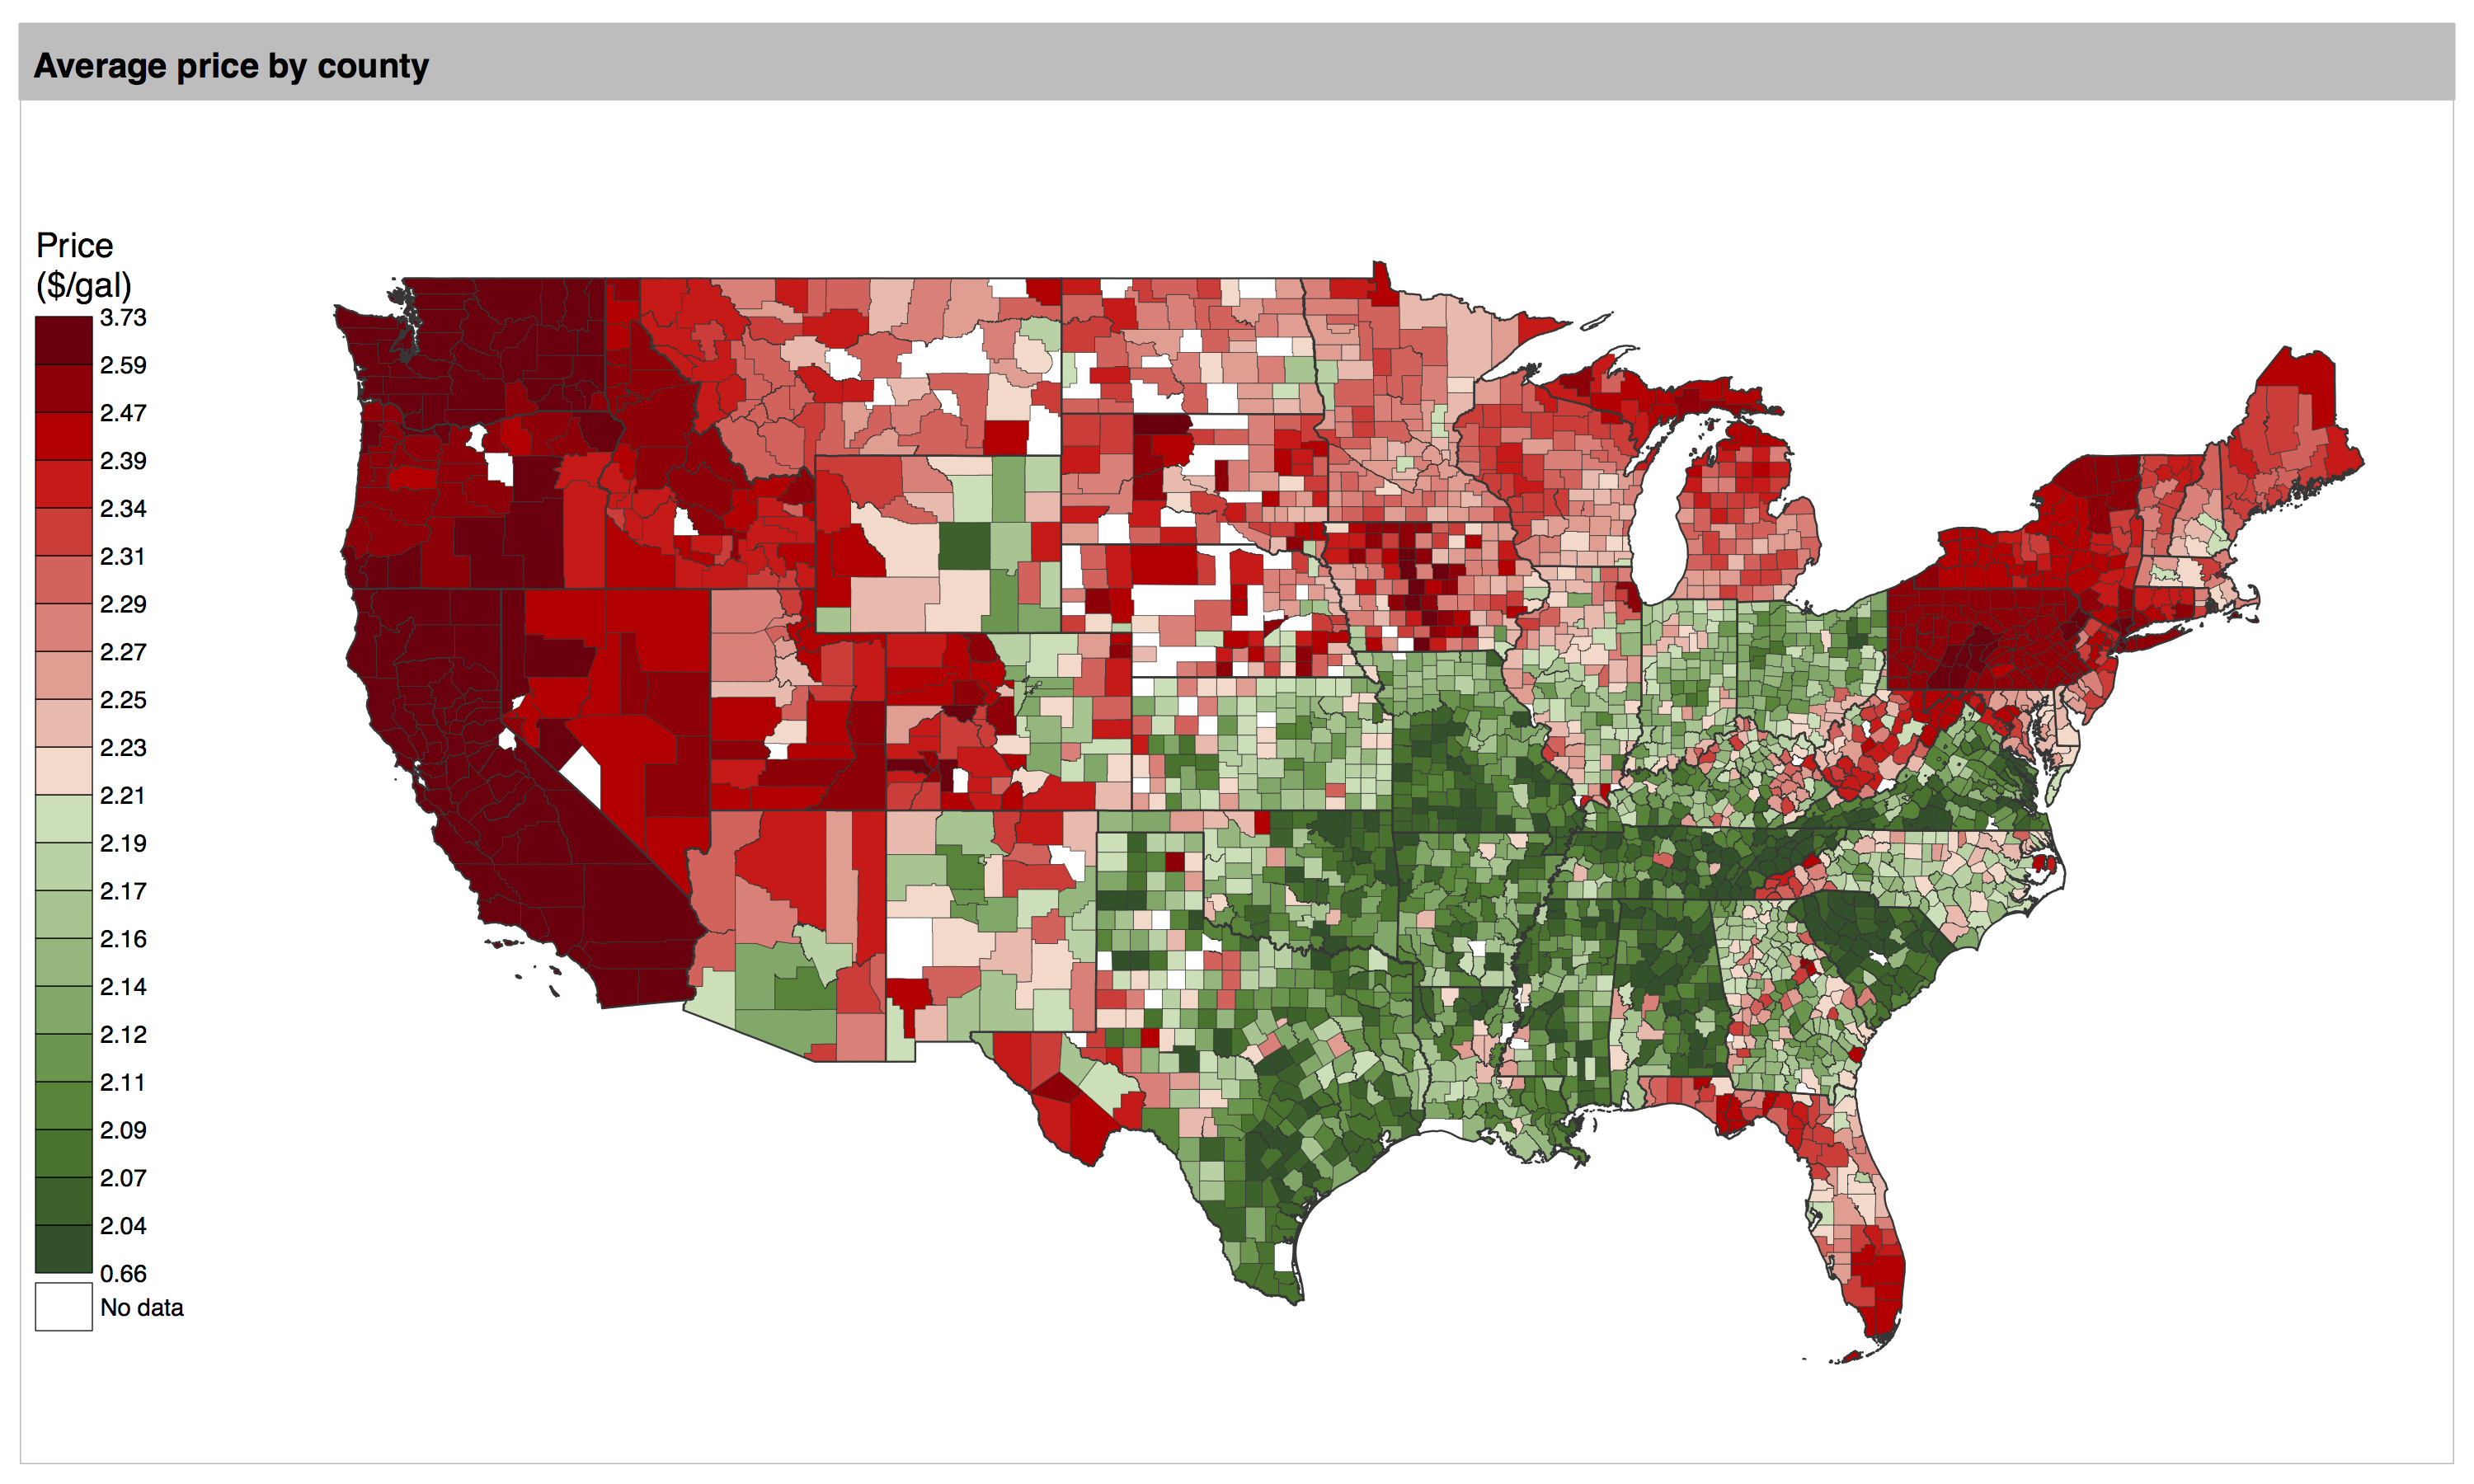
\includegraphics[width=\linewidth]{Figures/EnergyPrice/average_regular_map}
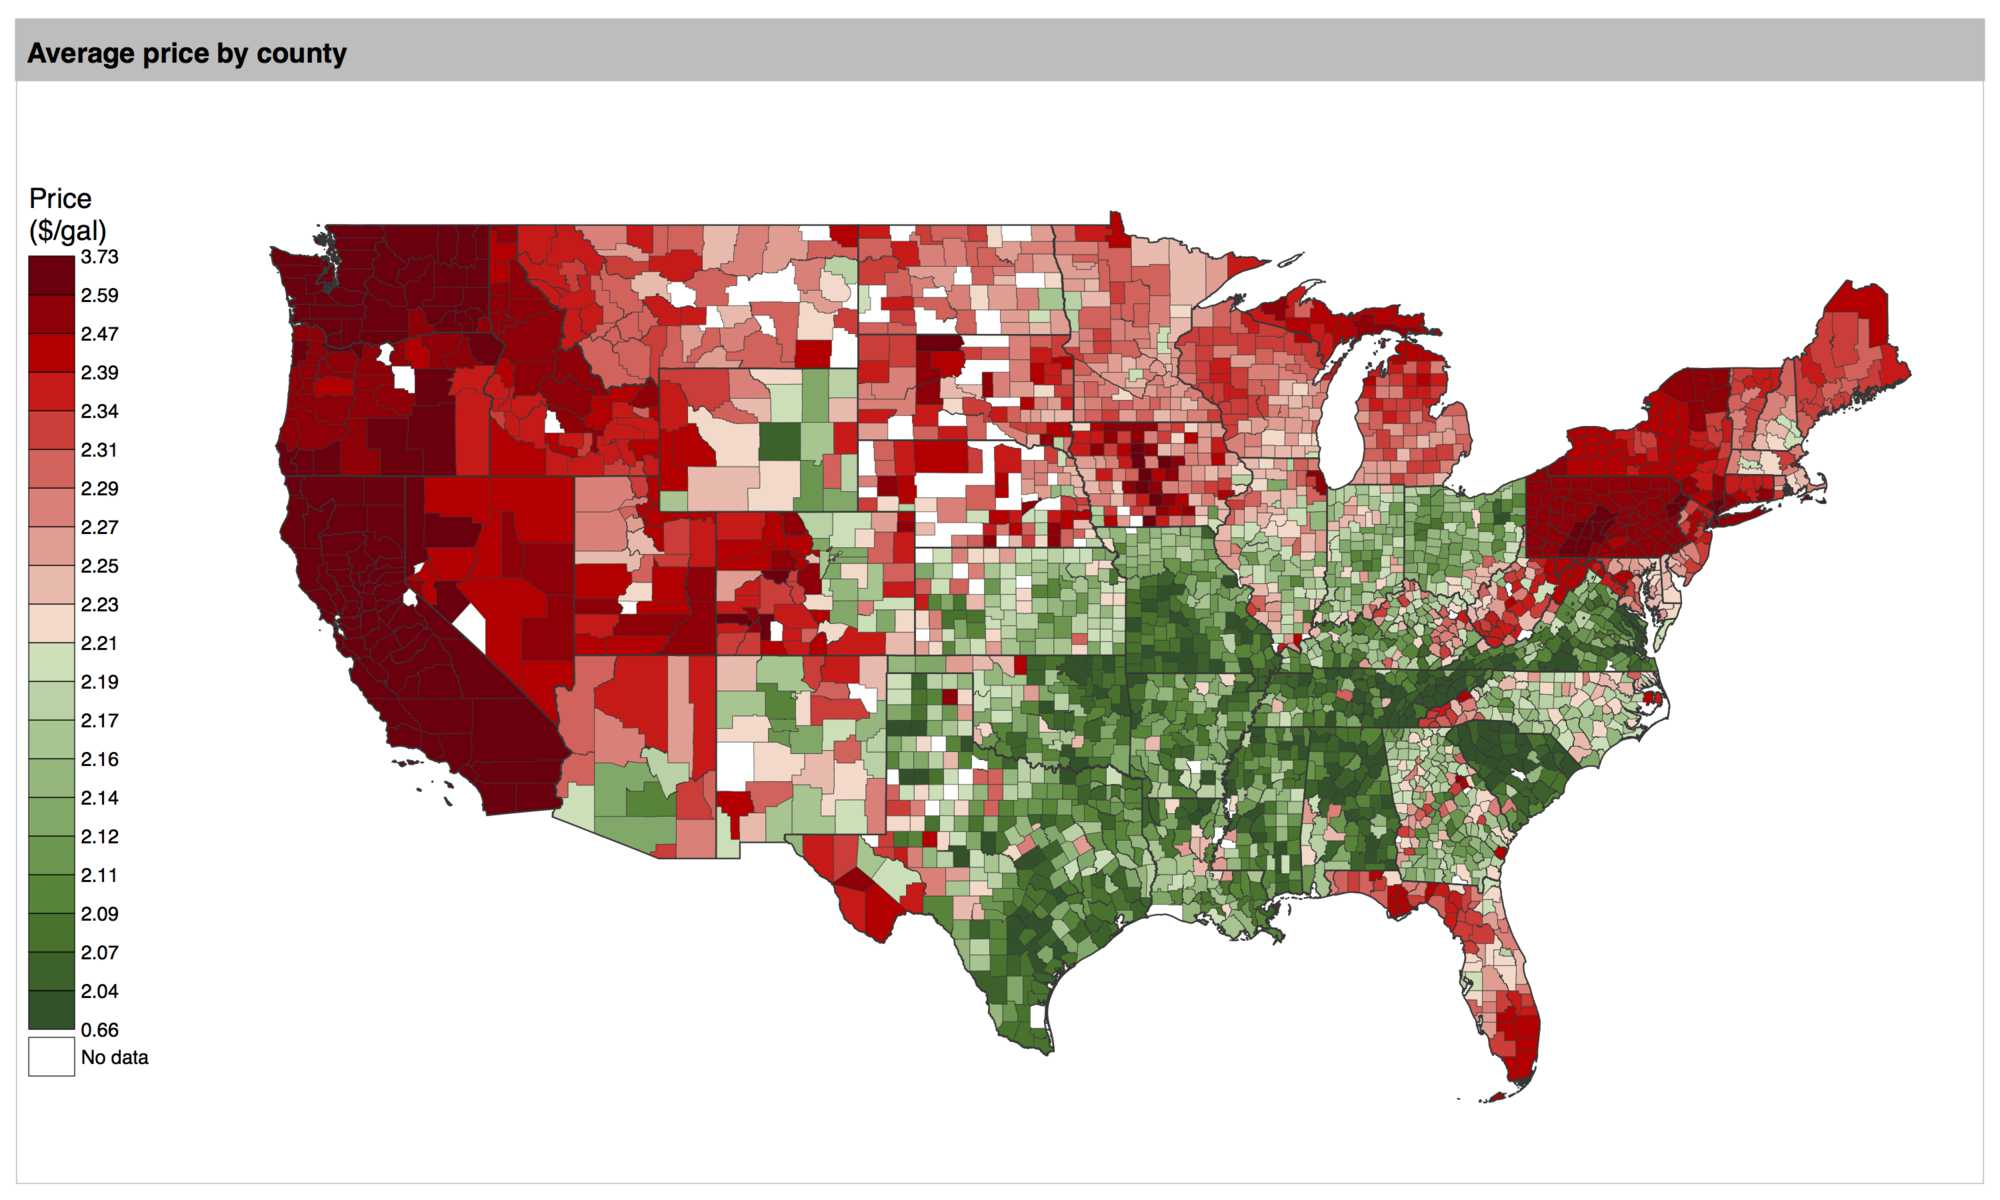
\includegraphics[width=\linewidth]{Figures/Final/8-2-2-fig-energyprice-map_price}
\caption[Mean price for counties][Prix moyen par Contés]{Map of mean price for counties, regular fuel, averaged over the whole period.\label{fig:energyprice:map_price}}{\textbf{Carte du prix moyen par comté.} Le prix est donné pour du carburant régulier, et la moyenne temporelle est prise sur l'ensemble de la période.\label{fig:energyprice:map_price}}
\end{figure}
%%%%%%%%%%%%%%%%%%%%%%


\bpar{
Since most of the variation in oil price is between gas station, we now focus mainly on spatial correlations. We will conduct the analysis at the county level for various reasons. First it appears that a variance decomposition of fuel price between and within county shows that more than 85\% of the variance is between-county, second because the localization of gas station is not reliable enough to allow for a smaller granularity and third because we have many socio-economic information at this level. We therefore study the spatial autocorrelation of prices at the county level. Spatial autocorrelation can be seen as an indicator of spatial heterogeneity which we measure using the Moran index~(\cite{tsai2005quantifying}), with spatial weights of the form $\exp{\left(-d_{ij} / d_0 \right)}$ with $d_{ij}$ being the distance between spatial entities $i$ and $j$, and $d_0$ a decay parameter giving the spatial range of interactions accounted for in the computation. We show in Fig.~\ref{fig:moran} its variations for each day and also as a function of the decay parameter. 
The fluctuations in time of the daily Moran index for low and medium spatial range, confirms geographical specificities in the sense of locally changing correlation regimes. These are logically smoothed for long ranges, as price correlations drop down with distance. The behavior of spatial autocorrelation with decay distance is particularly interesting: we observe a first regime change around 10km (from constant to piecewise linear regime), and a second important one around 1000km, both consistent across weekly time windows. We postulate that these correspond to typical spatial scales of the involved processes: the low regime would be local specificities and the middle one the state level processes. This behavior confirms that prices are non-stationary in space, and that therefore appropriate statistical techniques must be used to study potential drivers at different level. The two next subsections follow this idea and investigate potential explicative variables of local fuel prices, using two different techniques corresponding to two complementary paradigms: geographically weighted regression that puts the emphasis on neighborhood effects, and multi-level regression taking into account administrative boundaries.
}{
Puisque la majorité de la variation des prix est entre les stations, nous nous intéressons maintenant principalement aux corrélations spatiales. Nous conduisons l'analyse à l'échelle du Conté pour diverse raisons. D'une part une décomposition des prix des carburants inter et intra-Conté montre que plus de 85\% de la variance est inter-Conté, d'autre part car la localisation des stations n'est pas assez fiable pour permettre une granularité plus fine, et enfin car la majorité des variables socio-économiques est à ce niveau. Nous étudions donc l'autocorrelation spatiale des prix à l'échelle du Conté.

L'autocorrelation spatiale peut être vue comme une indicateur d'hétérogénéité spatiale que nous mesurons par l'index de Moran~(\cite{tsai2005quantifying}), avec des poids spatiaux de la forme $\exp{\left(-d_{ij} / d_0 \right)}$ avec  $d_{ij}$ étant la distance entre les entités spatiales $i$ et $j$, et $d_0$ un paramètre de décroissance donnant la portée spatiale des interactions que l'estimation prend en compte. Nous montrons en Fig.~\ref{fig:moran} ses variation pour chaque jour ainsi que comme fonction du paramètre de décroissance.

Les fluctuations dans le temps de l'index de Moran journalier pour les valeurs basses et moyennes du paramètre de decay, confirme les spécificité géographiques au sens de régimes de corrélation changeant localement. Celles-ci sont logiquement atténuées pour les longues portées, puisque les correlations des prix diminuent avec la distance. Le comportement de l'autocorrelation spatiale en fonction du paramètre de decay est particulièrement intéressant : nous observons une premier changement de régime atour de 10km (d'un régime constant à un régime linéaire par morceau), et une seconde transition importante autour de 1000km, les deux consistants sur des fenêtres temporelles à la semaine. Nous postulons que celles-ci correspondent au échelles spatiales typiques des phénomènes observés: le régime bas serait les spécificités locales et l'intermédiaire le processus au niveau de l'Etat.

Ce comportement confirme que les prix sont non-stationnaires dans l'espace, et que pour cette raison des techniques statistiques appropriées doivent être utilisées pour étudier les variables jouant un rôle à différents niveaux. Les deux parties suivantes suivent cette idée et étudient des variables explicatives potentielles des prix locaux du carburant, utilisant deux techniques différentes qui correspondent à deux paradigmes complémentaires : la régression géographique pondérée qui met l'emphase sur les effets de voisinage, et des régressions multi-niveaux prenant en compte les limites administratives.
}




%%%%%%%%%%%%%%
\begin{figure}
%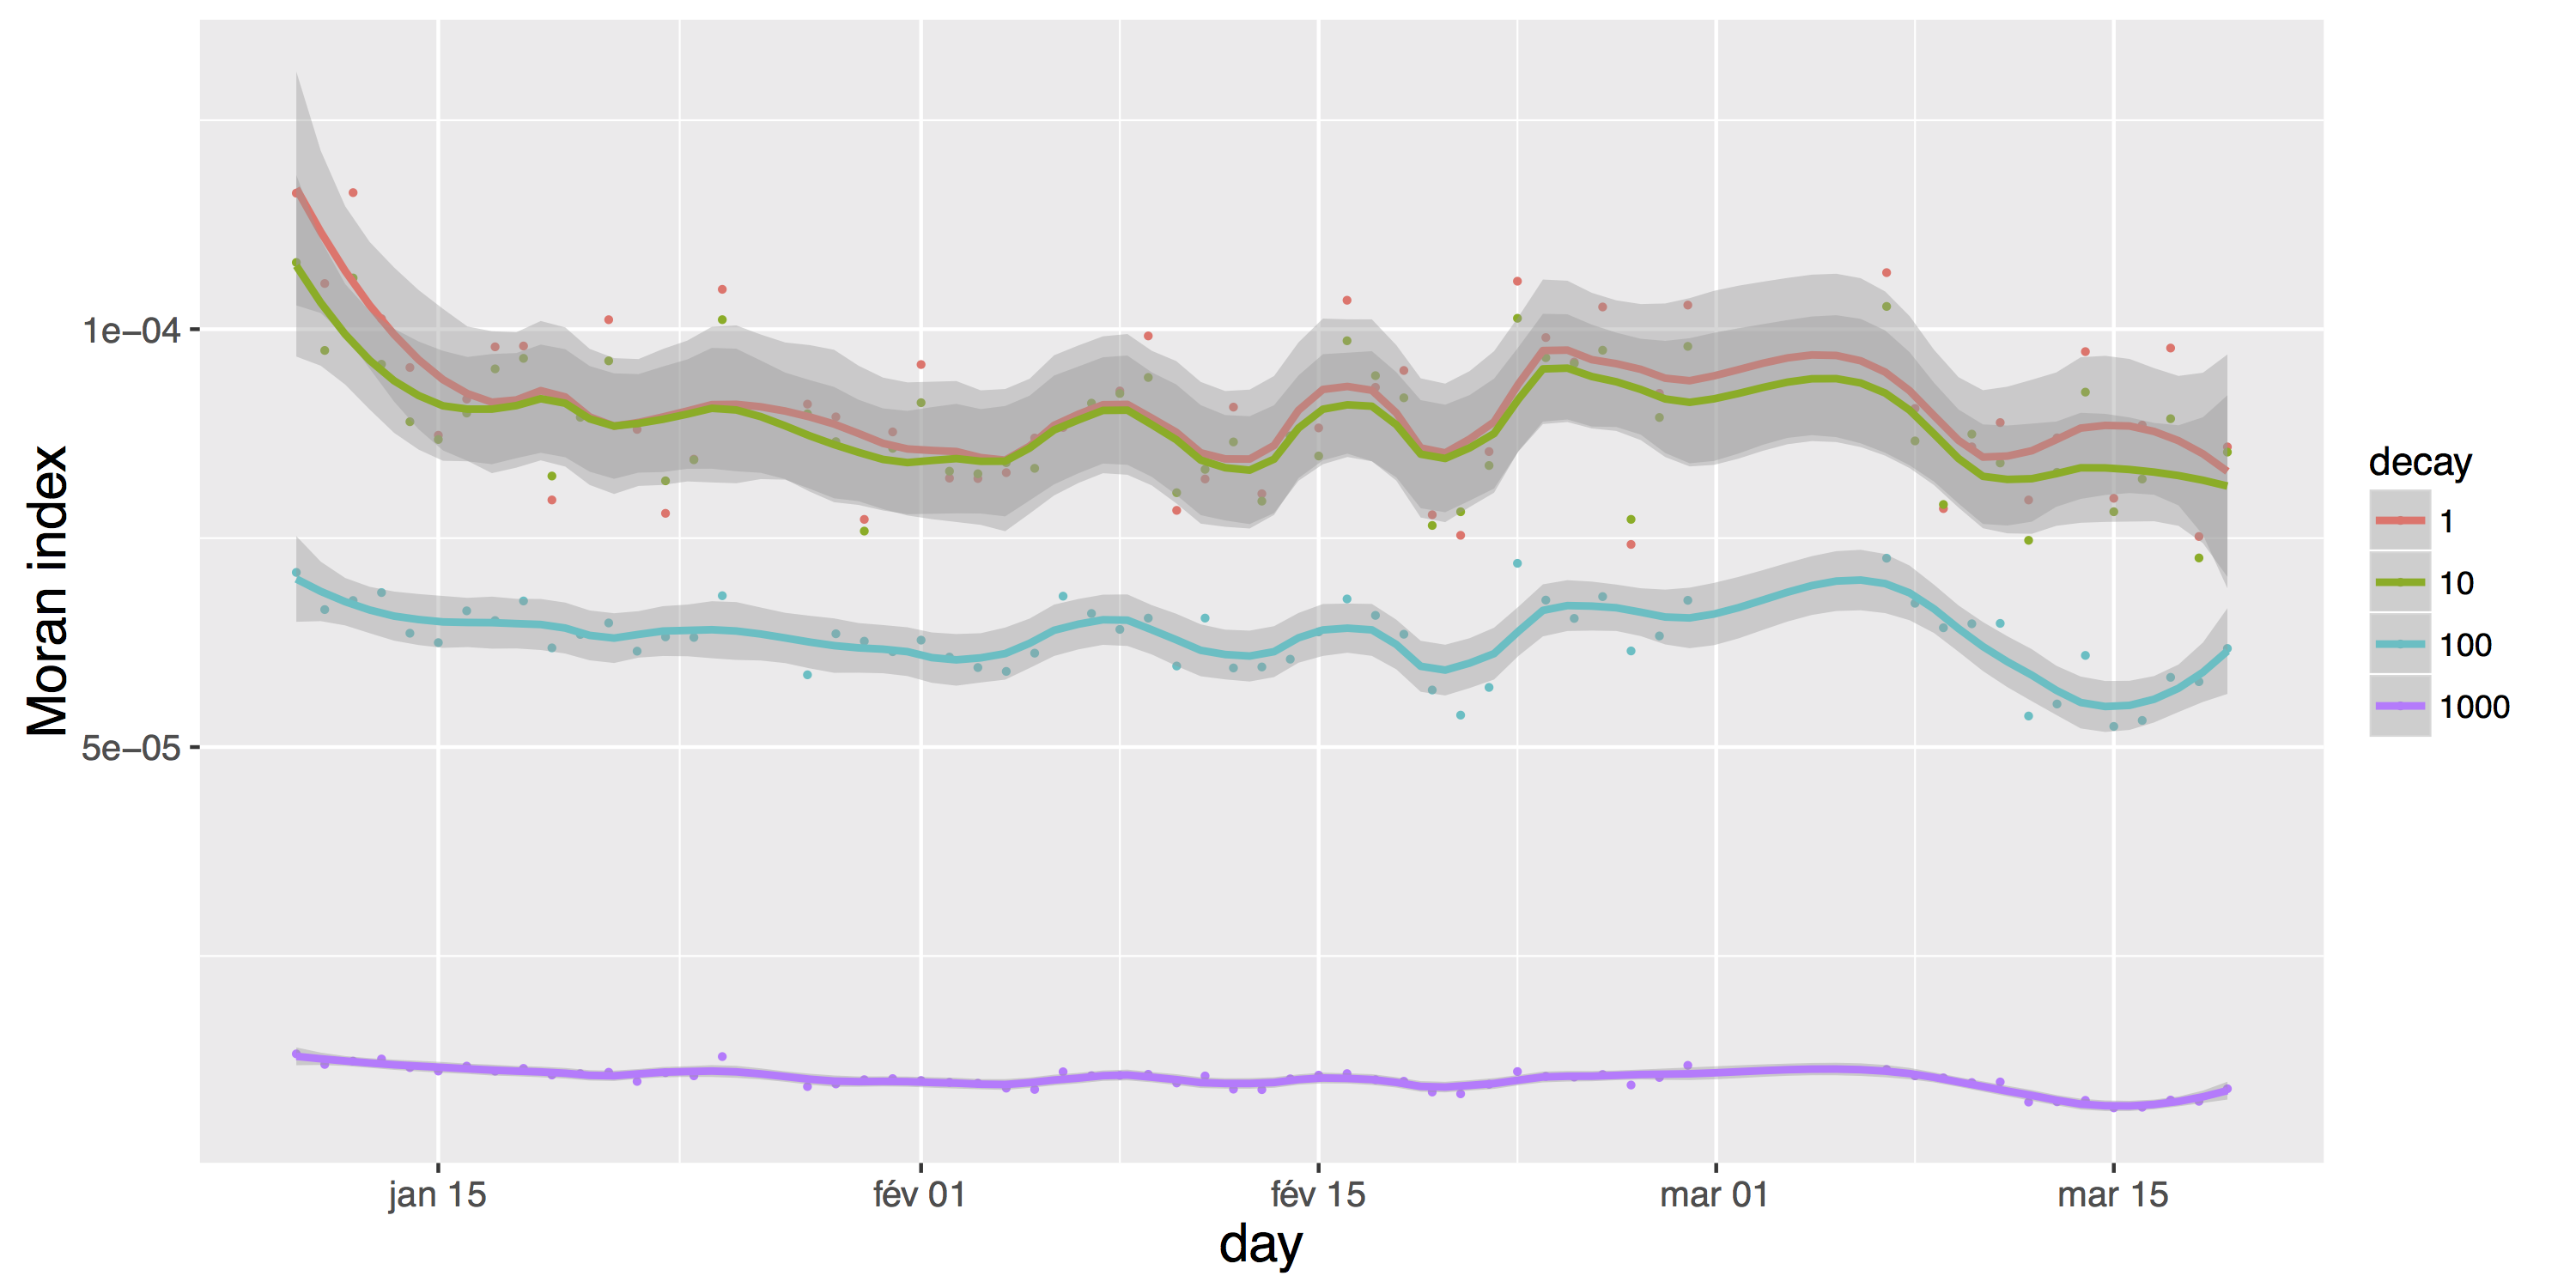
\includegraphics[width=\linewidth]{Figures/EnergyPrice/moran_days}\\
%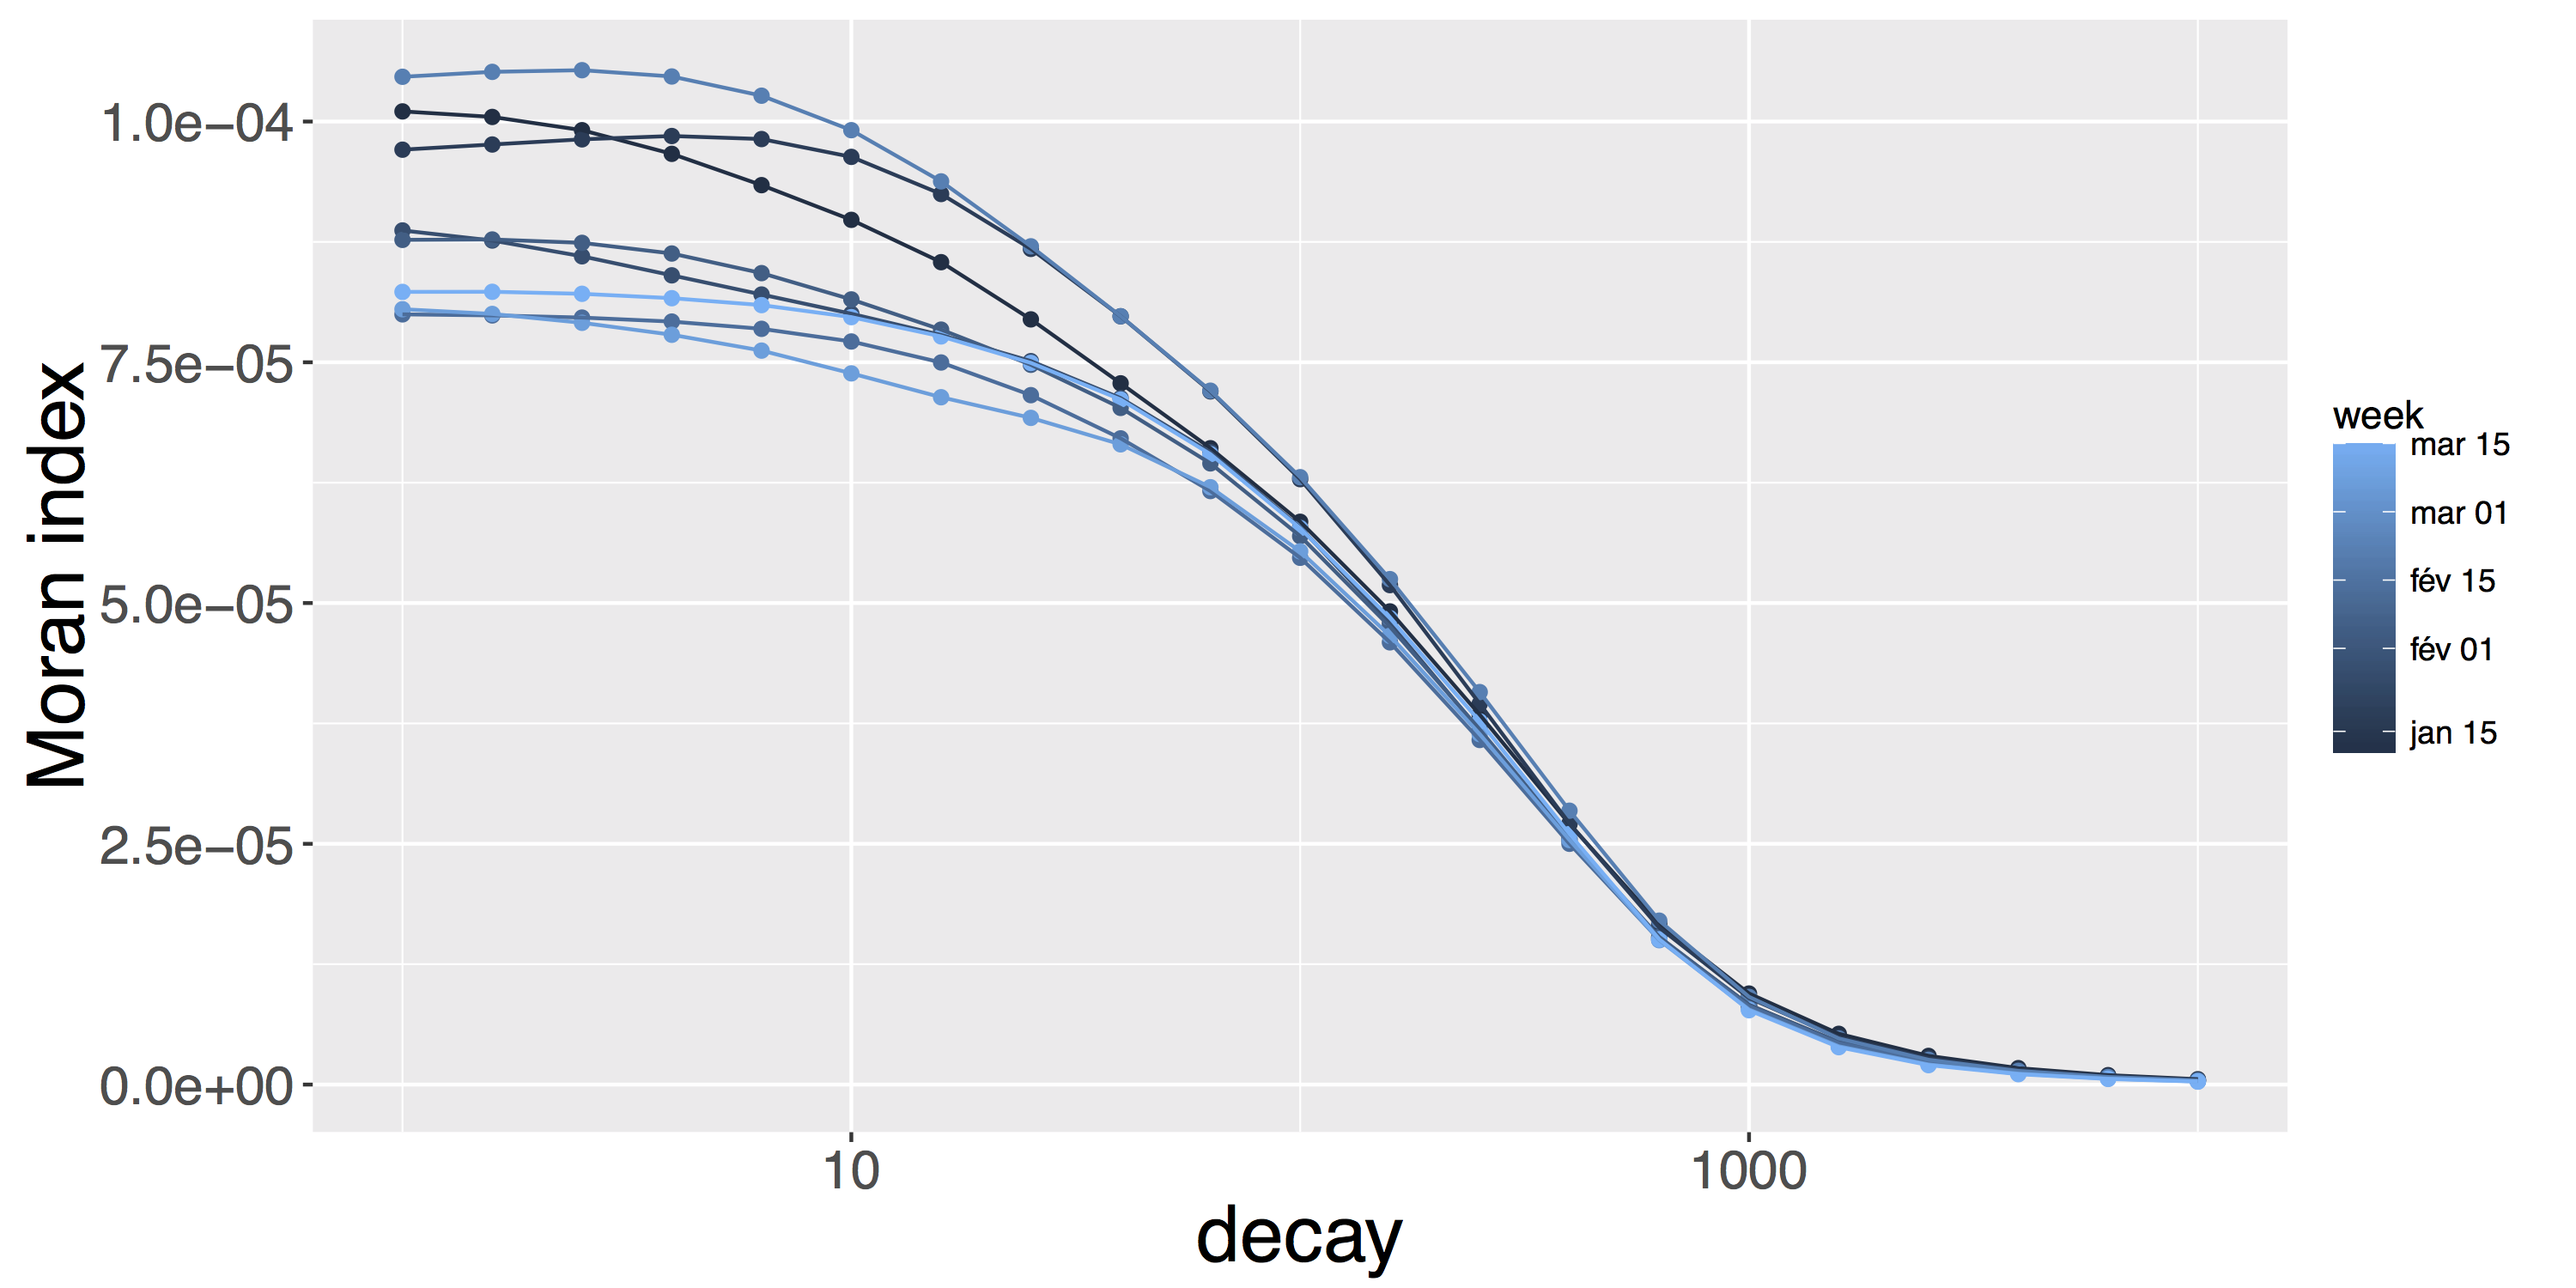
\includegraphics[width=\linewidth]{Figures/EnergyPrice/moran_decay_weeks}
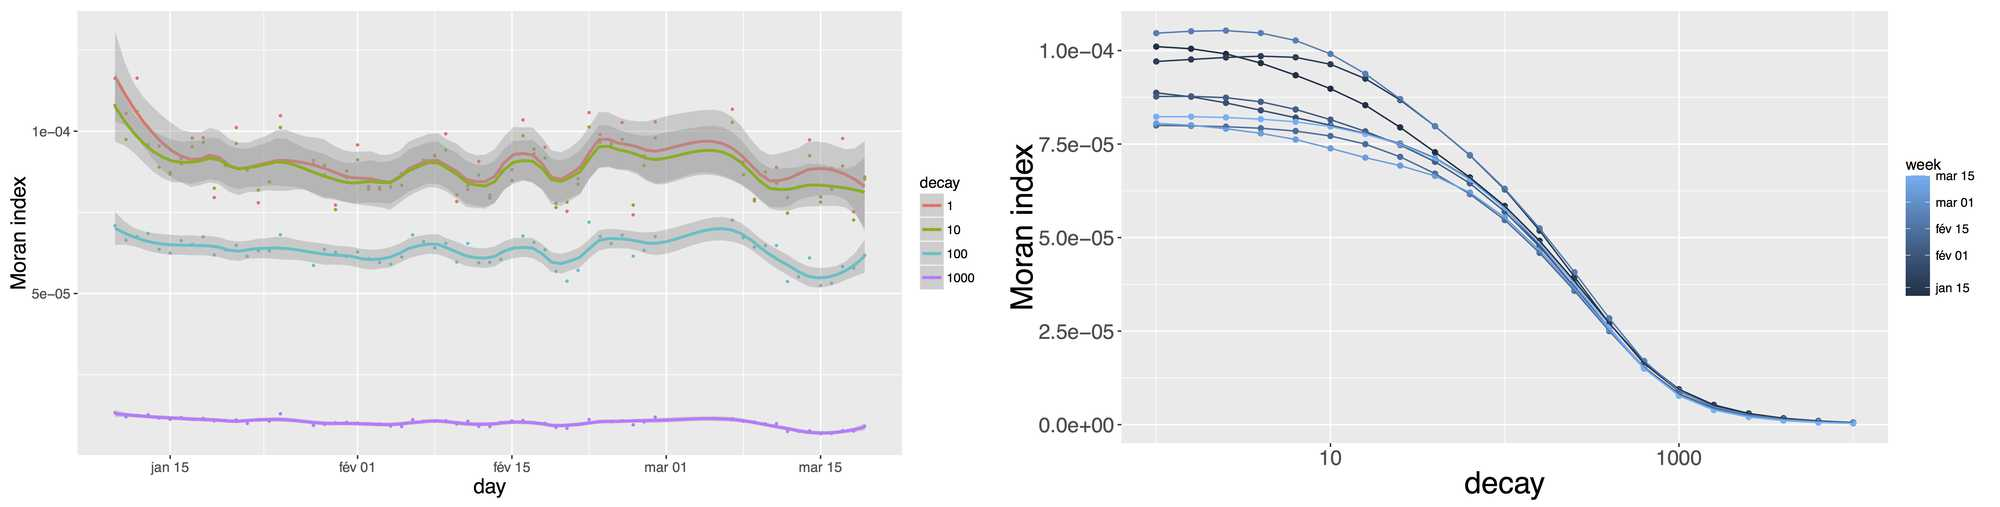
\includegraphics[width=\linewidth]{Figures/Final/8-2-2-fig-energyprice-moran.jpg}
\caption[Moran spatial-autocorrelation index][Autocorrelation spatiale]{\textbf{Behavior of Moran spatial-autocorrelation index.} (Left) Evolution in time of Moran index computed on daily time windows, for different decay parameter values. (Right) Moran index as a function of decay parameter, computed on weekly time windows.\label{fig:energyprice:moran}}{\textbf{Comportement de l'index d'autocorrelation spatiale de Moran.} (\textit{Gauche}) Evolution dans le temps de l'indice de Moran, calculé sur des fenêtres journalières, pour différentes valeurs du paramètre de décroissance. (\textit{Droite}) Indice de Moran en fonction du paramètre de décroissance, calculé sur des fenêtres hebdomadaires.\label{fig:energyprice:moran}}
\end{figure}
%%%%%%%%%%%%%%



\subsubsection{Geographically Weighted Regression}{Régression Géographique Pondérée}


\bpar{
The issue of spatial non-stationarity of geographical processes has always been a source of biased aggregated analyses or misinterpretations when applying general conclusions to local cases. To take it into account into statistical models, numerous techniques have been developed, among which the simple but very elegant Geographically Weighted Regression (GWR), that estimates non-stationary regressions by weighting observations in space similarly to kernel estimation methods. This was introduced in a seminal paper by~\cite{brunsdon1996geographically} and has been subsequently used and matured since then. The significant advantage of this technique is that an optimal spatial range in the sense of model performance can be inferred to derive a model that yields the effect of variables varying in space, thus revealing local effects that can occur at different spatial scales or across boundaries.
}{
La question de la non-stationnarité des processus géographiques a toujours été une source d'analyses agrégées biaisées ou de mauvaises interprétations lorsque des conclusions générales sont appliquées à des cas locaux. Pour le prendre en compte dans les modèles statistiques, de nombreuses techniques ont été proposées, parmi lesquelles la simple mais très élégante Régression Géographique Pondérée (GWR), qui estime des régressions non-stationnaires en pondérant les observations dans l'espace de manière similaire aux techniques d'estimation de densité par noyaux. Elle a été introduite dans un article séminal par \cite{brunsdon1996geographically} et a été utilisée et développée en conséquence depuis. L'avantage considérable de cette technique est qu'une portée spatiale optimale au sens de la performance du modèle peut être déduite pour dériver un modèle qui traduit des effets des variables variant dans l'espace, révélant ainsi des effets locaux qui peuvent se produire à différentes échelles spatiales ou à travers les frontières.
}

\bpar{
We proceed to multi-modeling to find the best model and associated kernel and spatial range. More specifically, we do the following: (i) we generate all possible linear models from the five potential variables (income, population, wage per job, jobs per capita, jobs); (ii) for each model and each candidate kernel shape (exponential, gaussian, bisquare, step), we determine the optimal bandwidth in the sense of both cross-validation and corrected Akaike Information Criterion (AICc) which quantifies information included in the model; (iii) we fit the models with this bandwidth. We choose the model with the best overall AICc, namely $price = \beta\cdot\left( income, wage, percapjobs\right)$ for a bandwidth of 22 neighbors and a gaussian kernel,\footnote{note that the kernel shape does not have much influence as soon as gradually decaying functions are used} with an AICc of $2,900$. The median AICc difference with all other models tested is 122. The global R-squared is 0.27, what is relatively good also compared to the best R-squared of 0.29 (obtained for the model with all variables, which clearly overfits with an AICc of 3010; furthermore, effective dimension is less than 5 as 90\% of variance is explained by the three first principal components for the normalized variables).
}{
Nous procédons à une multi-modélisation pour trouver le meilleur modèle ainsi que le noyau et la portée spatiale optimaux associés. Plus précisément, nous suivons les étapes suivantes : (i) tous les modèles linéaires potentiels à partir des cinq variables candidates sont générés (revenu, population, salaire par emploi, emploi par tête, emplois); (ii) pour chaque modèle et chaque forme de noyau candidate (exponentiel, gaussien, bisquare, escalier), nous déterminons la portée optimale au sens à la fois de la cross-validation et du critère d'Information d'Akaike corrigé (AICc) qui quantifie l'information contenue dans le modèle; (iii) nous ajustons les modèles avec cette portée. Nous choisissons le modèle avec le meilleur AICc, en l'occurence $price = \beta\cdot\left( income, wage, percapjobs\right)$ pour une portée de 22 voisins et un noyau Gaussien,\footnote{Nous notons que la forme du noyau n'a pas plus d'influence tant que des fonctions décroissant graduellement sont utilisées.} avec un AICc de $2,900$. La différences médiane d'AICc avec l'ensemble des autre modèles est 122. Le coefficient de détermination global est 0.27, ce qui est relativement bon en comparaison du meilleur R$^2$ de 0.29 (obtenu pour le modèle avec l'ensemble des variables, qui sur-ajuste clairement avec un AICc de 3010; de plus la dimension effective est inférieure à 5 puisque 90\% de la variance est expliquée par les trois premières composantes principales pour les variables normalisées.
}


\bpar{
The coefficients and local R-squared for the best model are shown in Fig.~\ref{fig:gwr}. The spatial distribution of residuals (not shown here) seems globally randomly distributed, which confirms in a way the consistency of the approach. Indeed, if a distinguishable geographical structure had been found in the residuals, it would have meant that the geographical model or the variable considered had failed to translate spatial structure. Let now turn to an interpretation of the spatial structures we obtain. First of all, the spatial distribution of the model performance reveals that regions where these simple socio-economic factors explain do a good job in explaining prices are mostly located on the west coast, the south border, the north-east region from lakes to the east coast, and a stripe from Chicago to the south of Texas. The corresponding coefficients have different behaviors across the areas, suggesting different regimes.\footnote{We comment their behavior in areas where the model has a minimal performance, that we fix arbitrarily as a local R-squared of 0.5} For example, the influence of income in each region seems to be inverted when the distance to the coast increases (from north to south-east in the west, south to north in Texas, east to west in the east), what may be a fingerprint of different economic specializations. On the contrary, the regime shifts for wage show a clear cut between west (except around Seattle) and middle/east, that does not correspond to state-policies only as Texas splits in two. The same way, jobs per capita show an opposition between east and west, what could be due for example to cultural differences. These results are difficult to interpret directly, and must be understood as a confirmation that geographical particularities matters, as regions differ in regimes of role for each of the simple socio-economic-variables. Further precise knowledge could be obtained through targeted geographical studies including qualitative field studies and quantitative analyses, that are beyond the scope of this exploratory paper and left for further research.
}{
Les coefficients et le R$^2$ local pour le meilleur modèle sont montrés en Fig.~\ref{fig:energyprice:gwr}. La distribution spatiales des résidus (qui n'est pas montrée ici), semble globalement distribuée aléatoirement, ce qui confirme d'une certaine façon la cohérence de l'approche. En effet, si une structure géographique distinguable était trouvée dans les résidus, cela signifierait que le modèle géographique ou les variables considérées ont échoués à traduire la structure spatiale.

Nous pouvons à présent proposer une interprétation des structures spatiales obtenues. Tout d'abord, la distribution spatiale de la performance du modèle révèle des régions où ces indicateurs socio-économiques simples expliquent relativement bien les prix, et celles-ci sont localisées sur la côte ouest, la frontière sud, la région nord-est des lacs à la côte est, et une bande de Chicago au sud du Texas. Les coefficients correspondants ont des comportements différents selon les zones, suggérant différents régimes\footnote{Nous commentons leur comportement dans les zones où le modèle a une performance minimale, que nous fixons arbitrairement à un R2 local de 0.5.}.

Par exemple, l'influence du revenu dans chaque région semble s'inverser quand la distance à la côte augmente (du nord au sud-est dans l'ouest, du sud au nord au Texas, de l'est à l'ouest dans l'est), ce qui pourrait témoigner de différentes spécialisations économiques. Au contraire, le changement de régime pour les salaires montre une rupture notable entre l'ouest (sauf autour de Seattle) et le centre et l'est, qui ne correspond pas directement à des politiques d'Etat locales puisque le Texas est coupé en deux par exemple. De la même façon, les emplois par capita montrent une opposition entre est et ouest, qui pourrait être due par exemple à des différences culturelles.

Ces résultats sont toutefois difficiles à interpréter directement, et doivent être compris comme la confirmation que les particularités géographiques importent, puisque les régions diffèrent dans le régime du rôle de chacune des variables socio-économiques simples. Une connaissance plus précise pourrait être obtenue par des études géographiques ciblées incluant des études de terrain qualitatives et des analyses quantitatives, qui sont au delà de la portée de cette étude exploratoire et laissée à une éventuelle recherche future.
}


\bpar{
Finally, we extract the spatial scale of the studied processes, that is, by computing the distribution of distance to nearest neighbors with the optimal bandwidth. It yields roughly a log-normal distribution, of median 77km and interquartile 30km. We interpret this scale as the spatial stationarity scale of price processes in relation with economic agents, which can also be understood as a range of coherent market competition between gas stations.
}{
Enfin, nous extrayons l'échelle spatiale des processus étudies, c'est à dire en calculant la distribution de la distance aux plus proches voisins avec la portée optimale. On obtient approximativement une distribution log-normale, de médiane 77km et d'interquartile 30km. Nous interprétons cette échelle comme l'échelle de stationnarité spatiale du processus de prix en relation avec les agents économiques, qui peut également être comprise comme la portée des marchés cohérents de compétition entre les station service.
}



%%%%%%%%%%%%%%%
\begin{figure}
%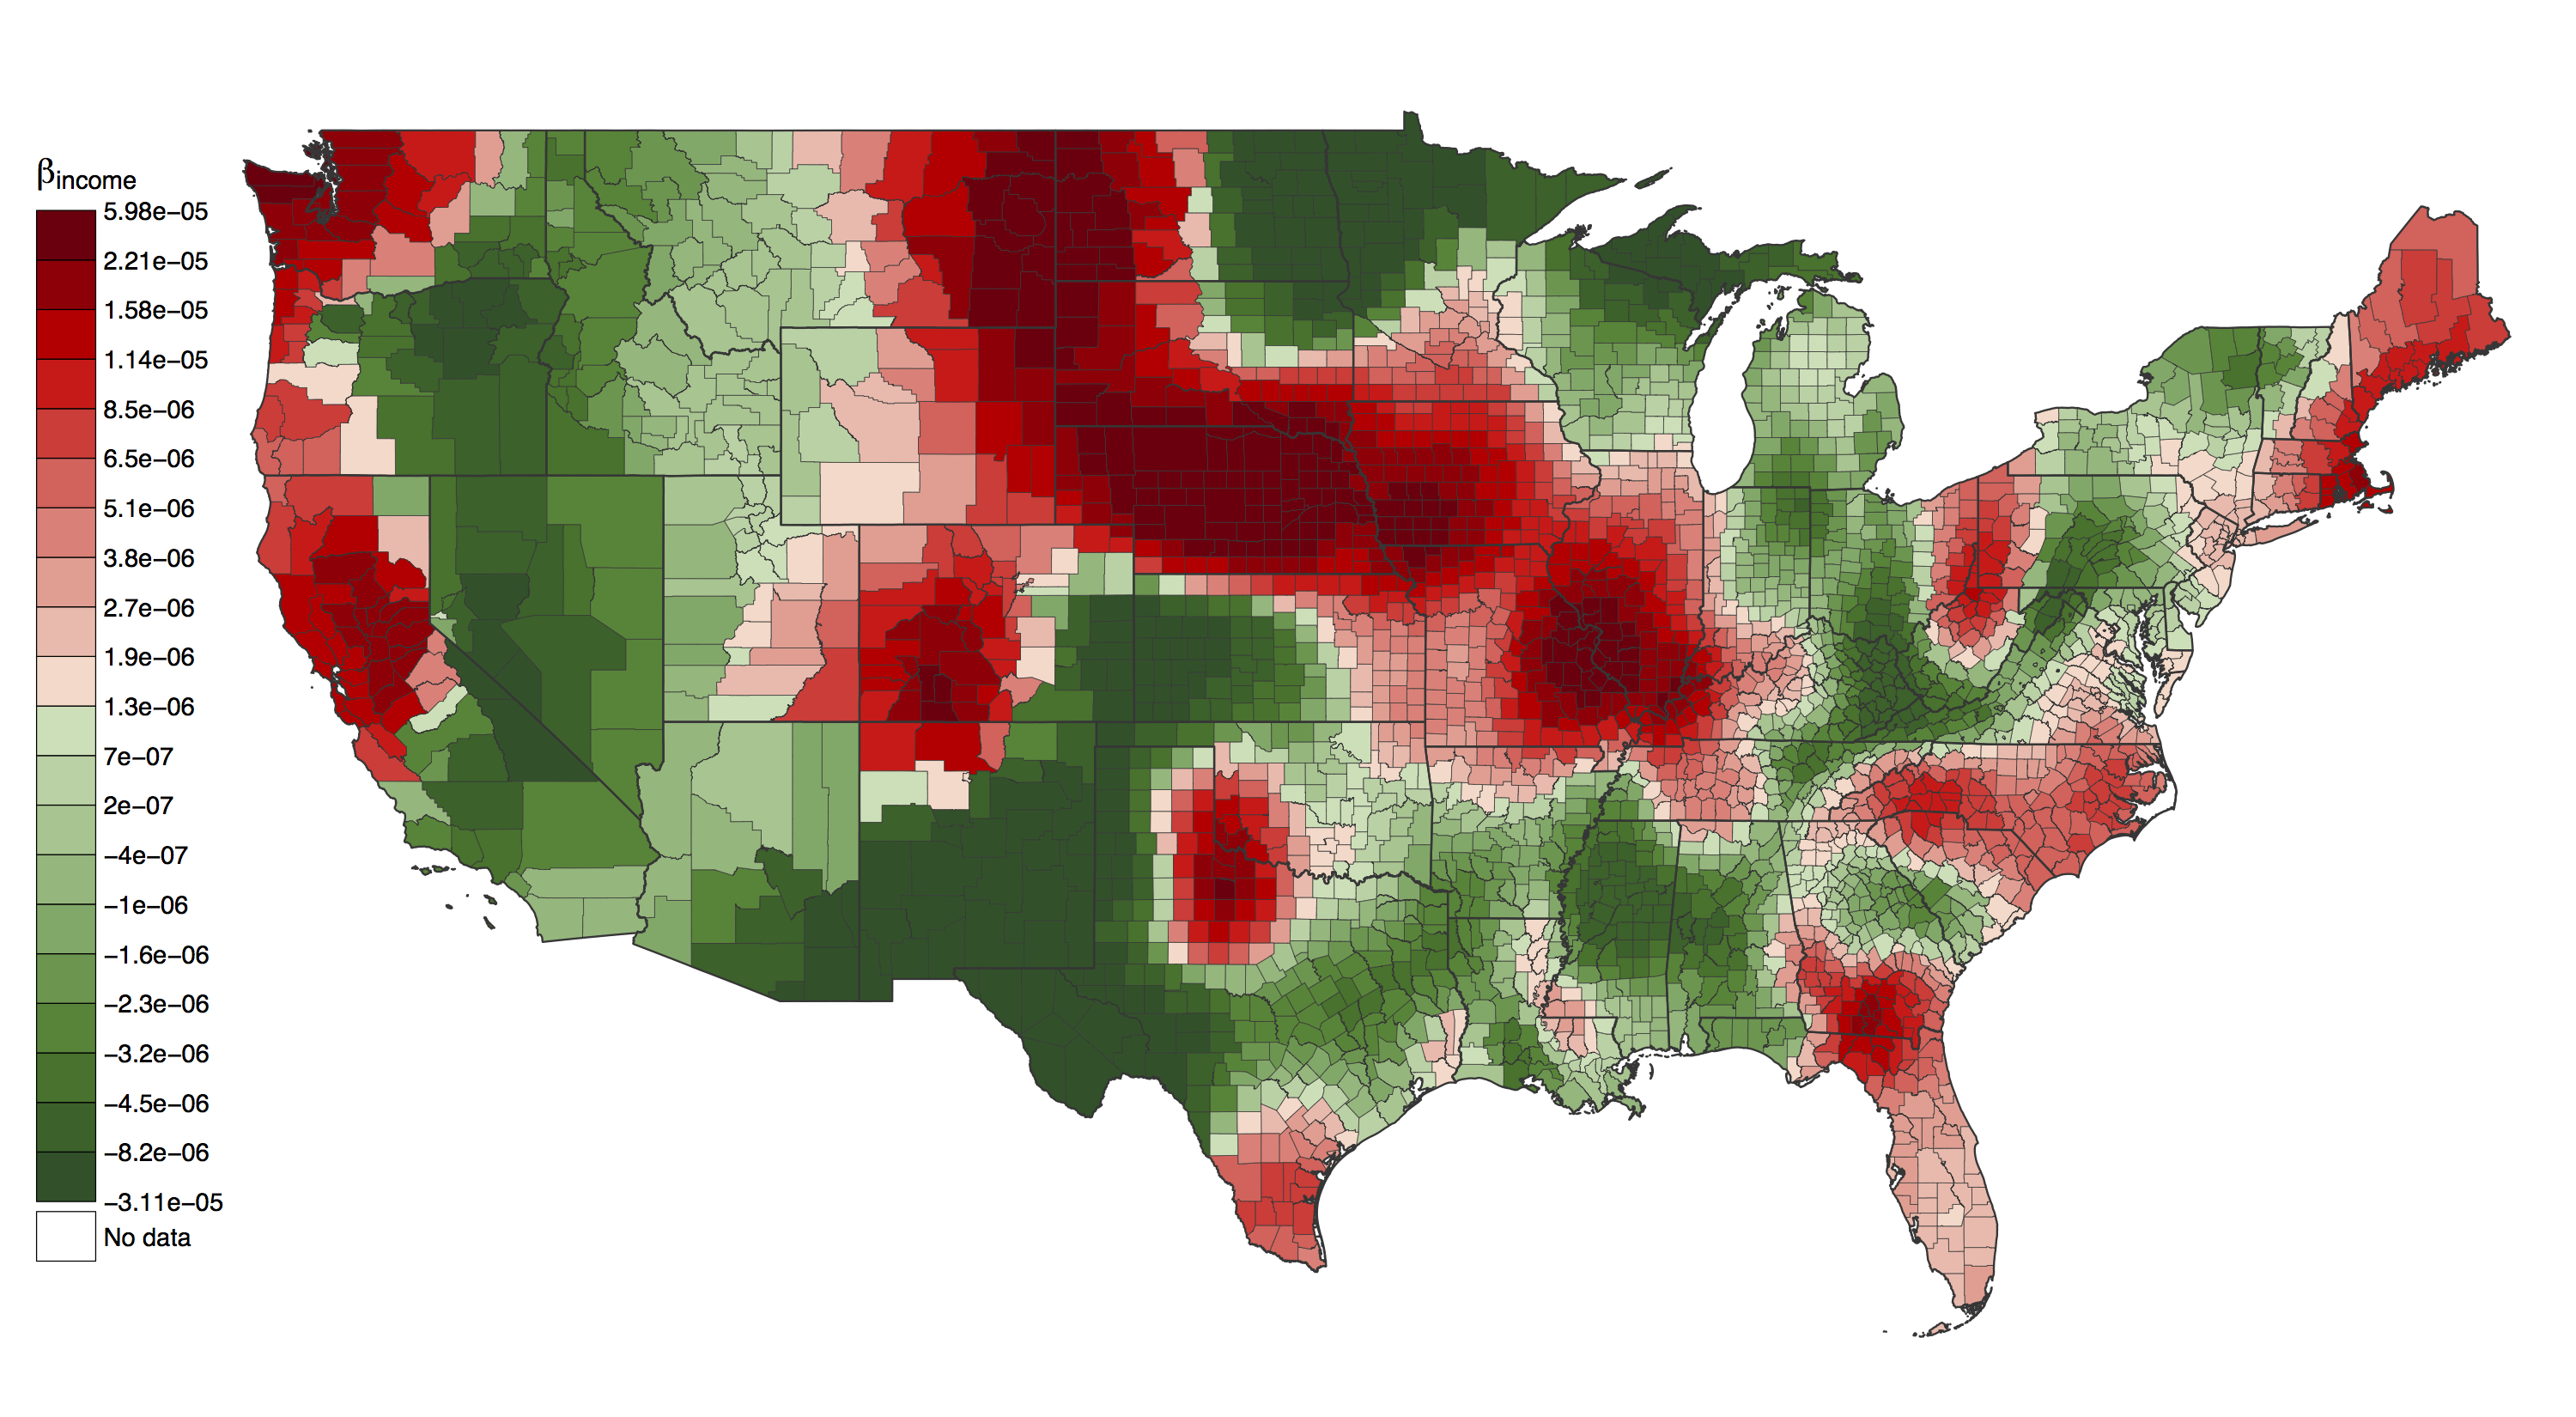
\includegraphics[width=0.49\linewidth]{Figures/EnergyPrice/gwr_allbest_betaincome}
%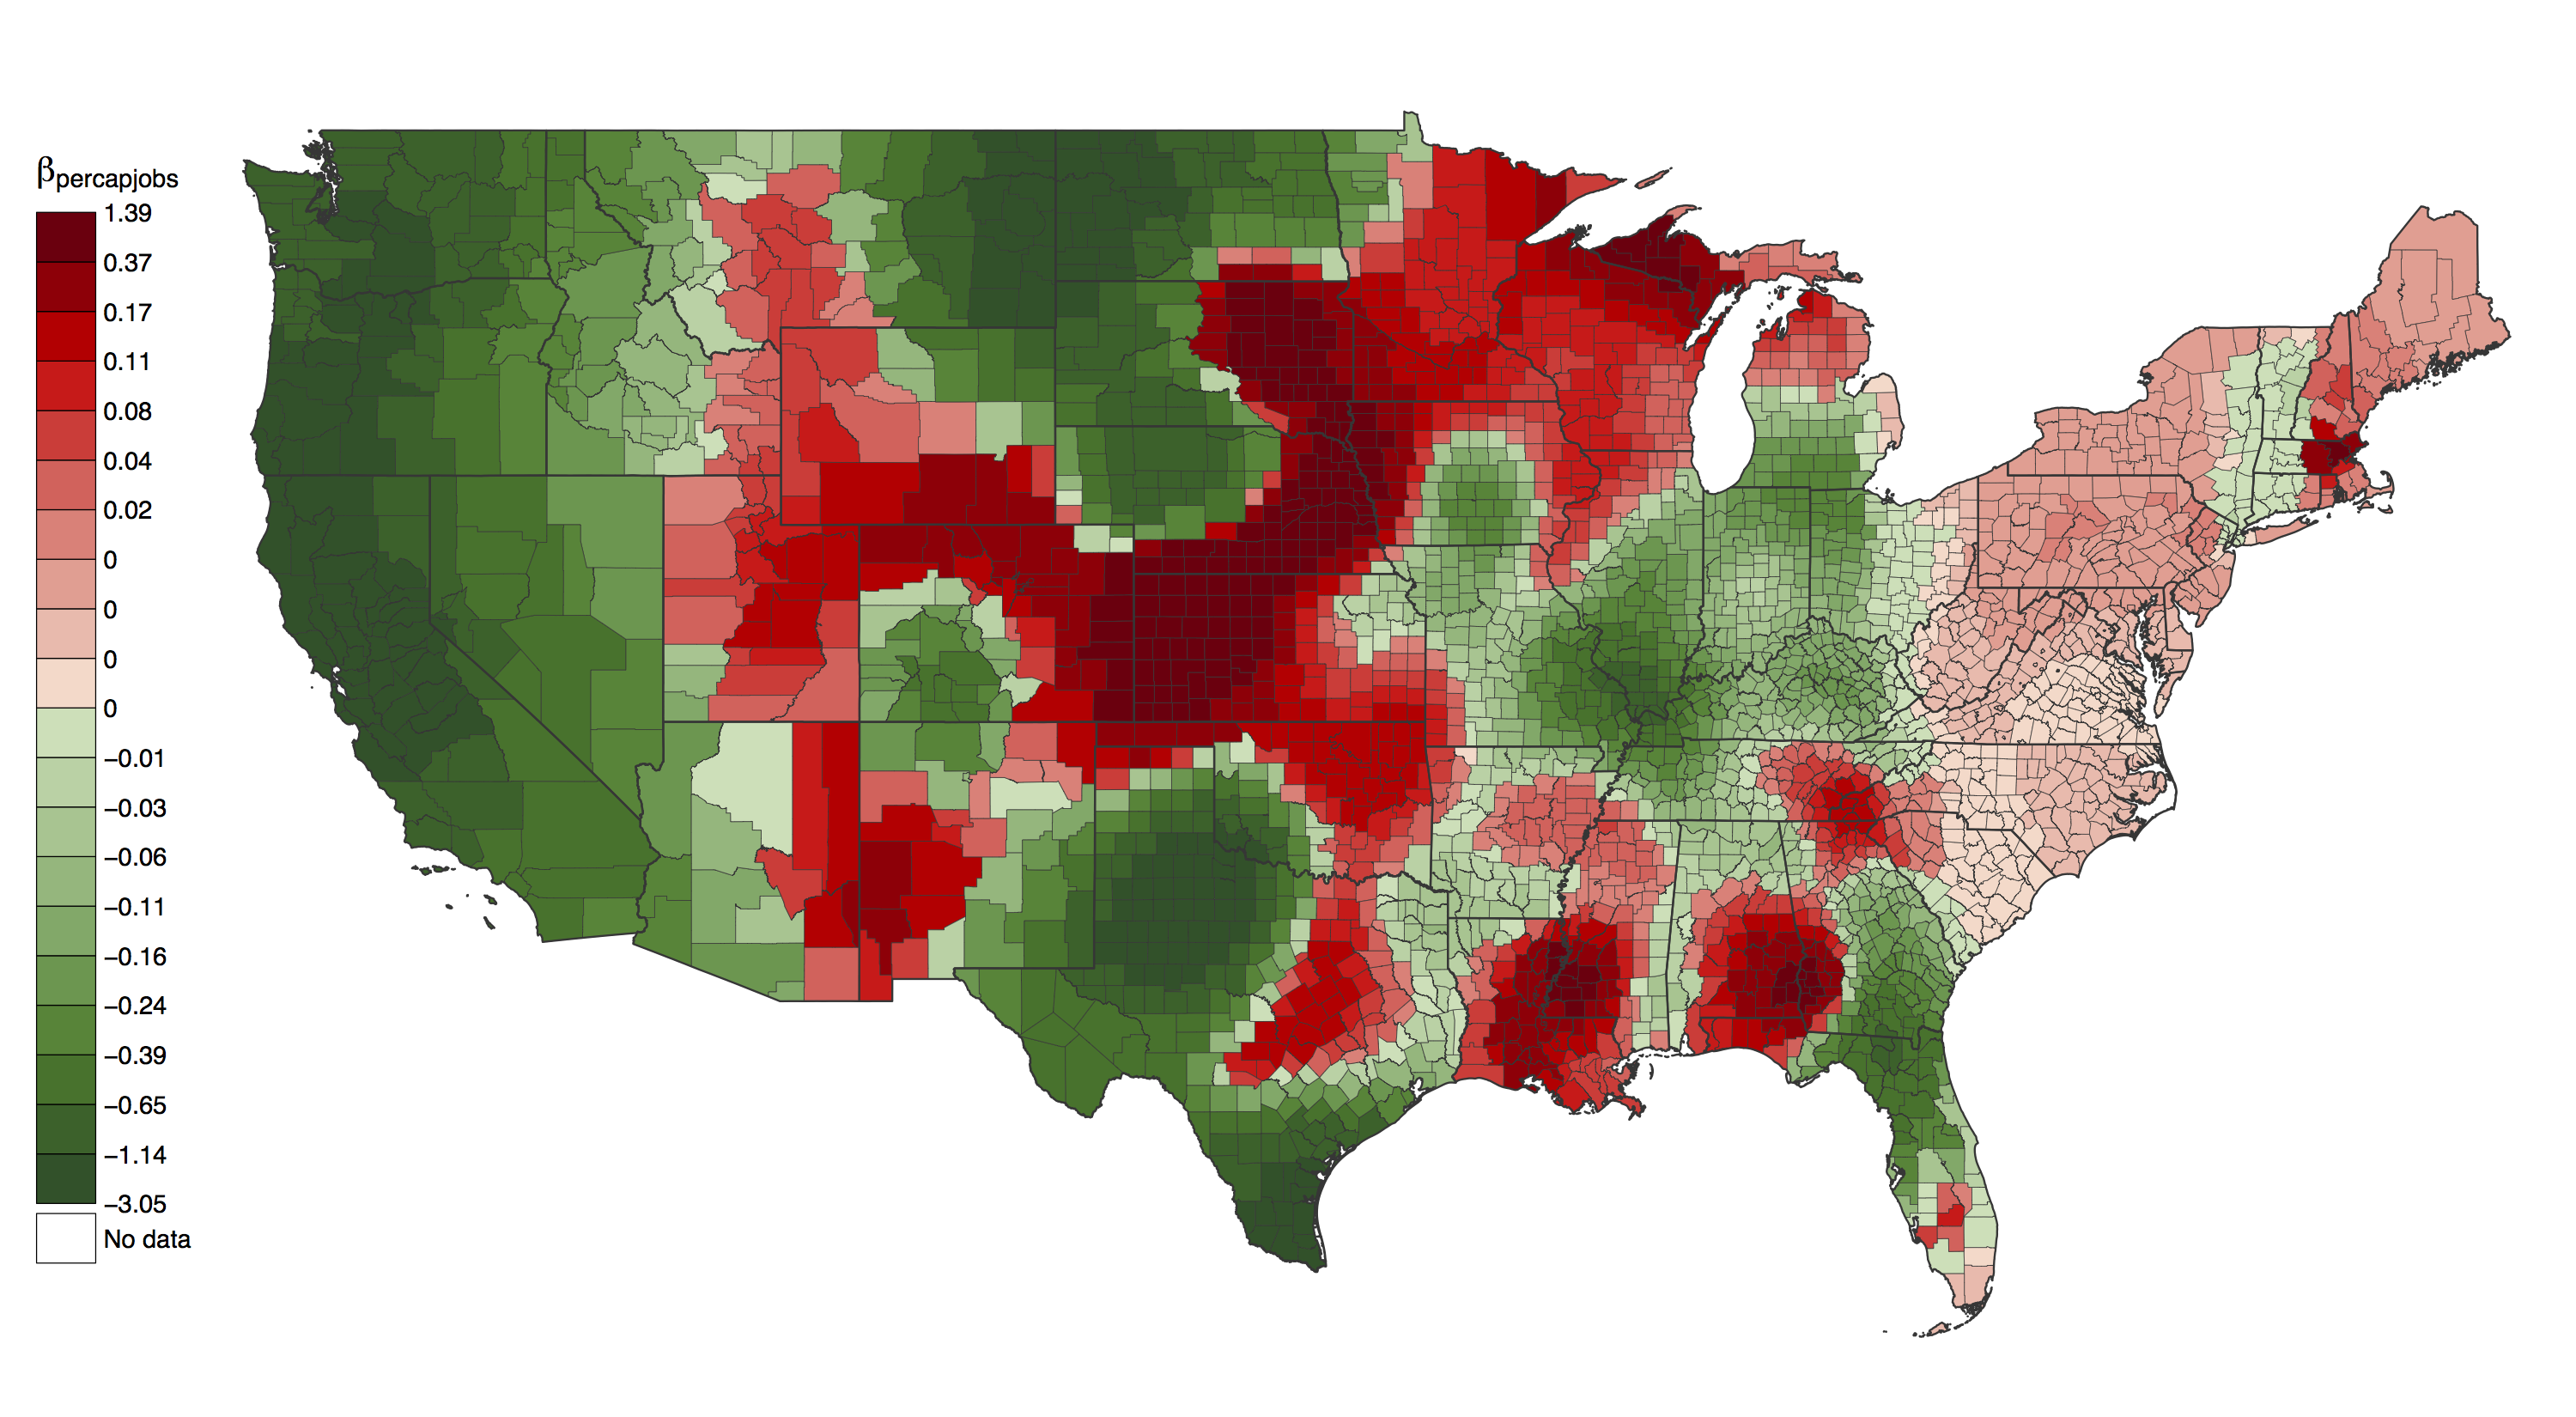
\includegraphics[width=0.49\linewidth]{Figures/EnergyPrice/gwr_allbest_betapercapjobs}\\
%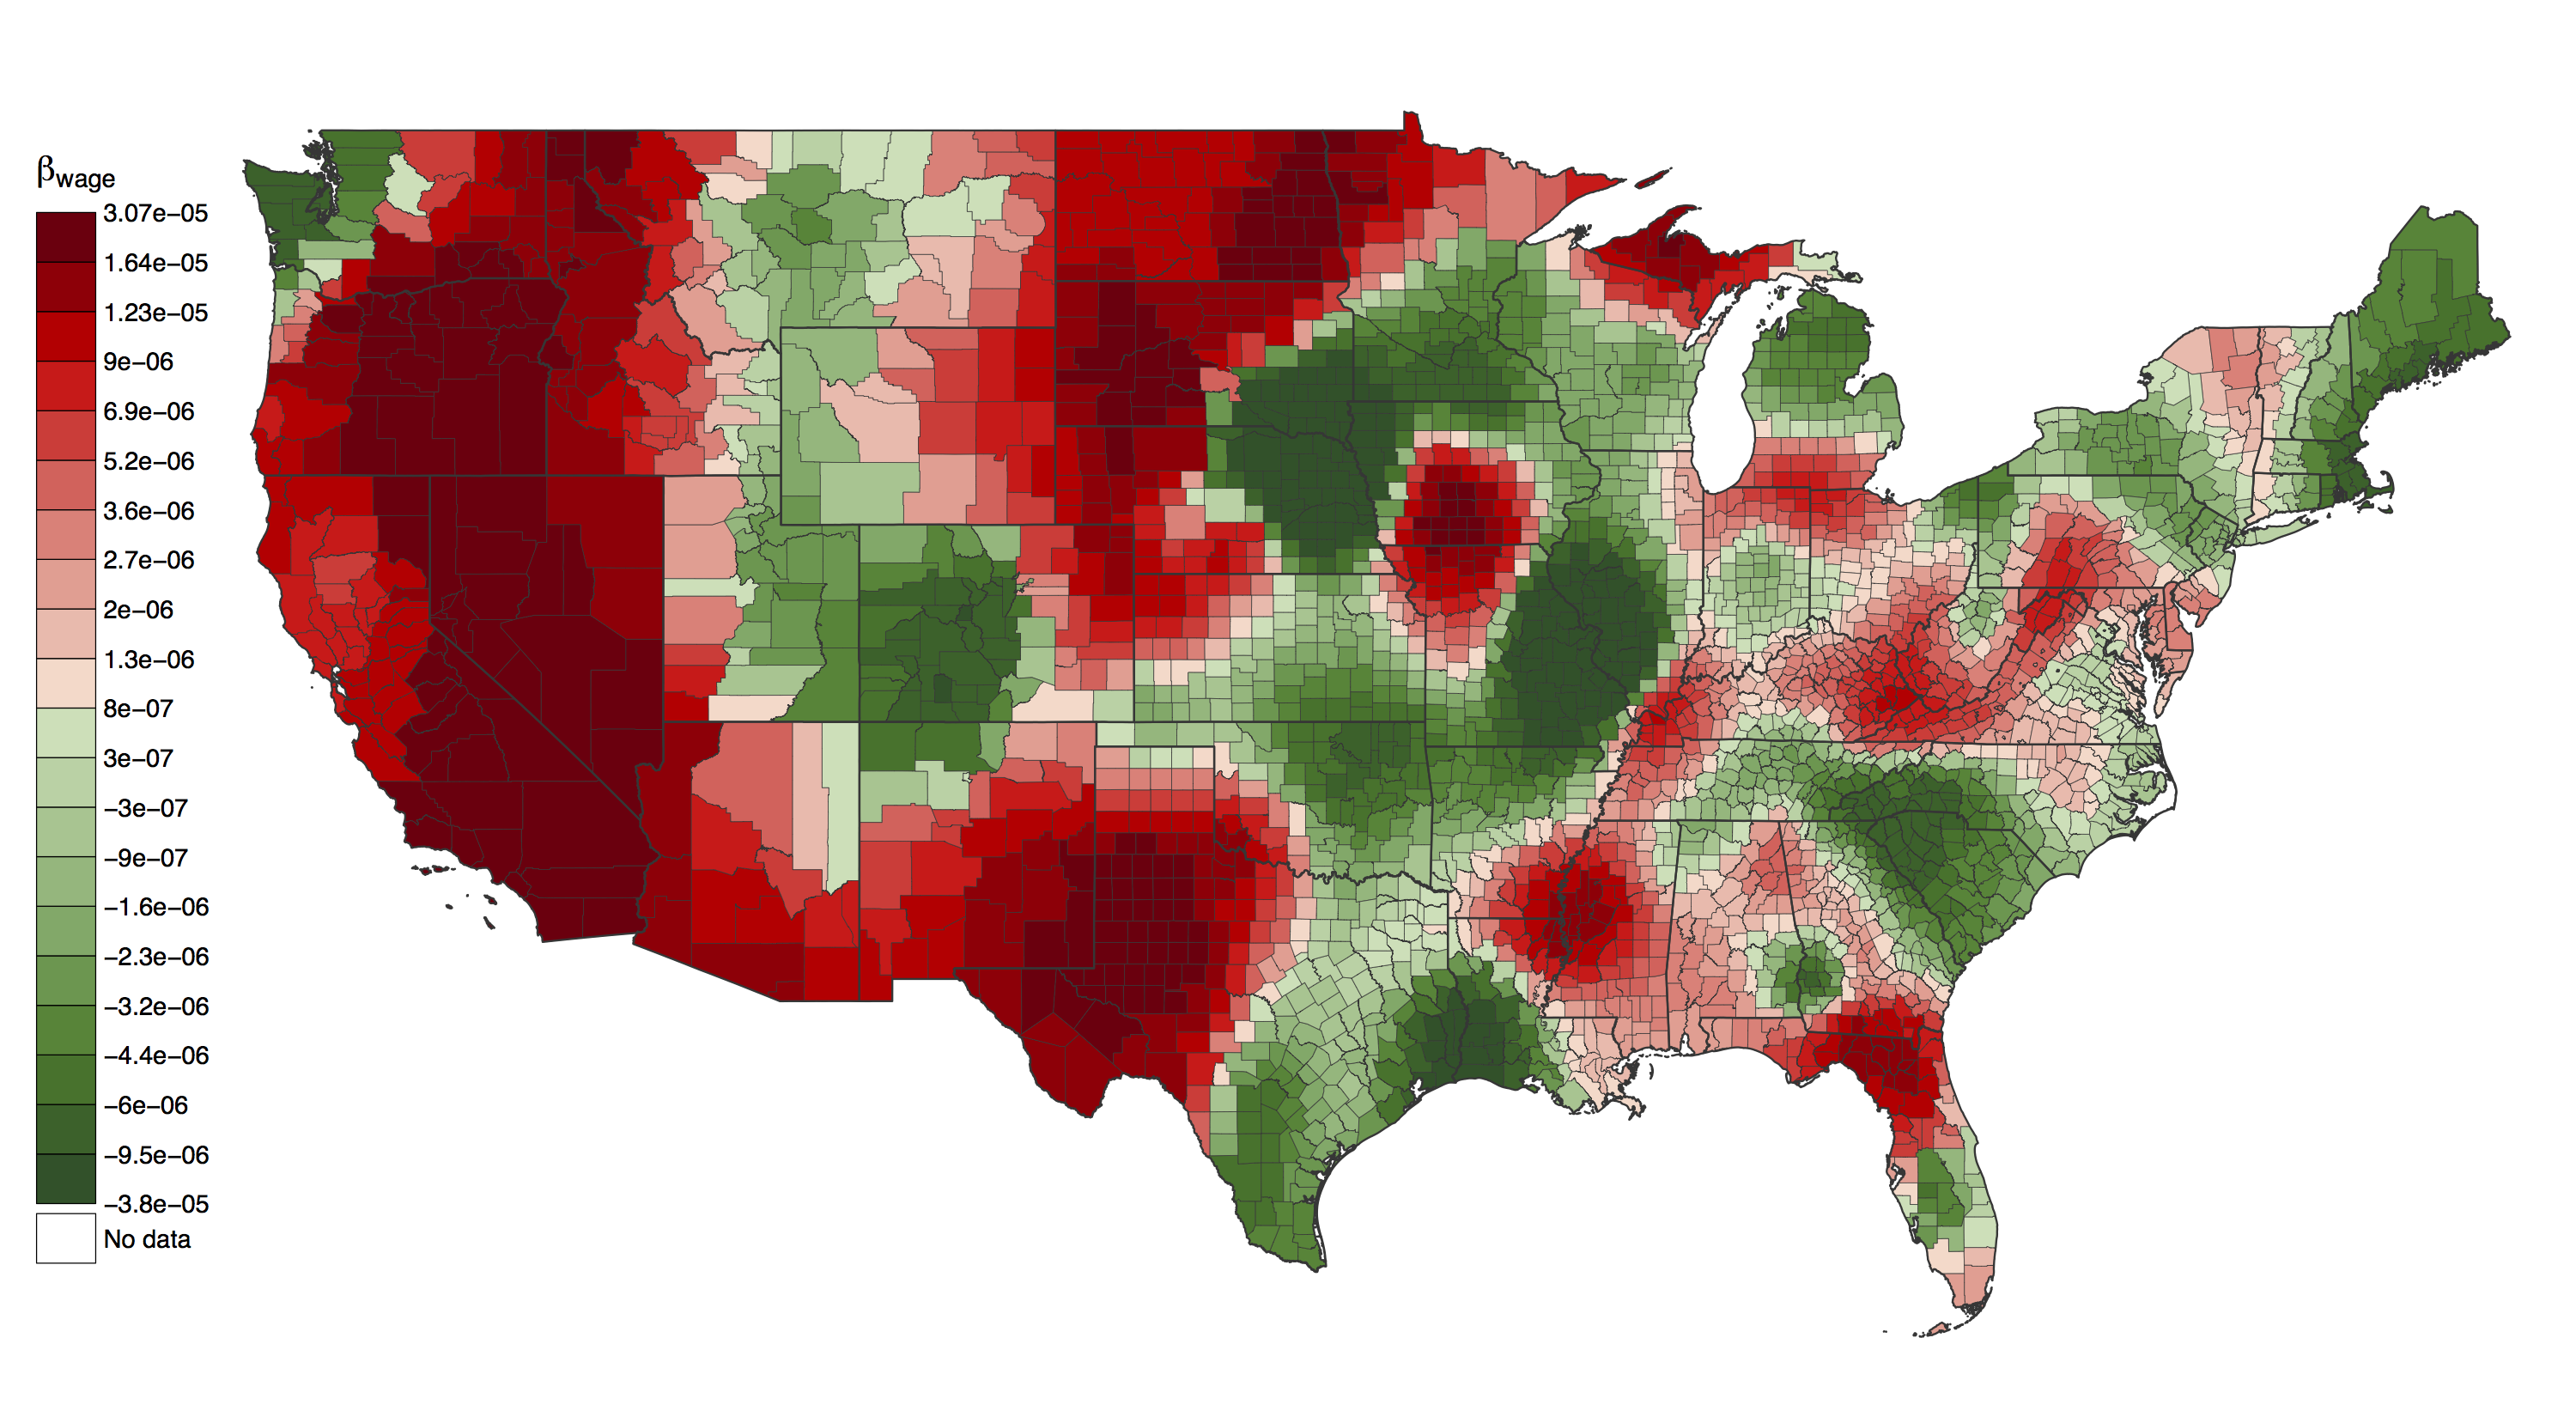
\includegraphics[width=0.49\linewidth]{Figures/EnergyPrice/gwr_allbest_wage}
%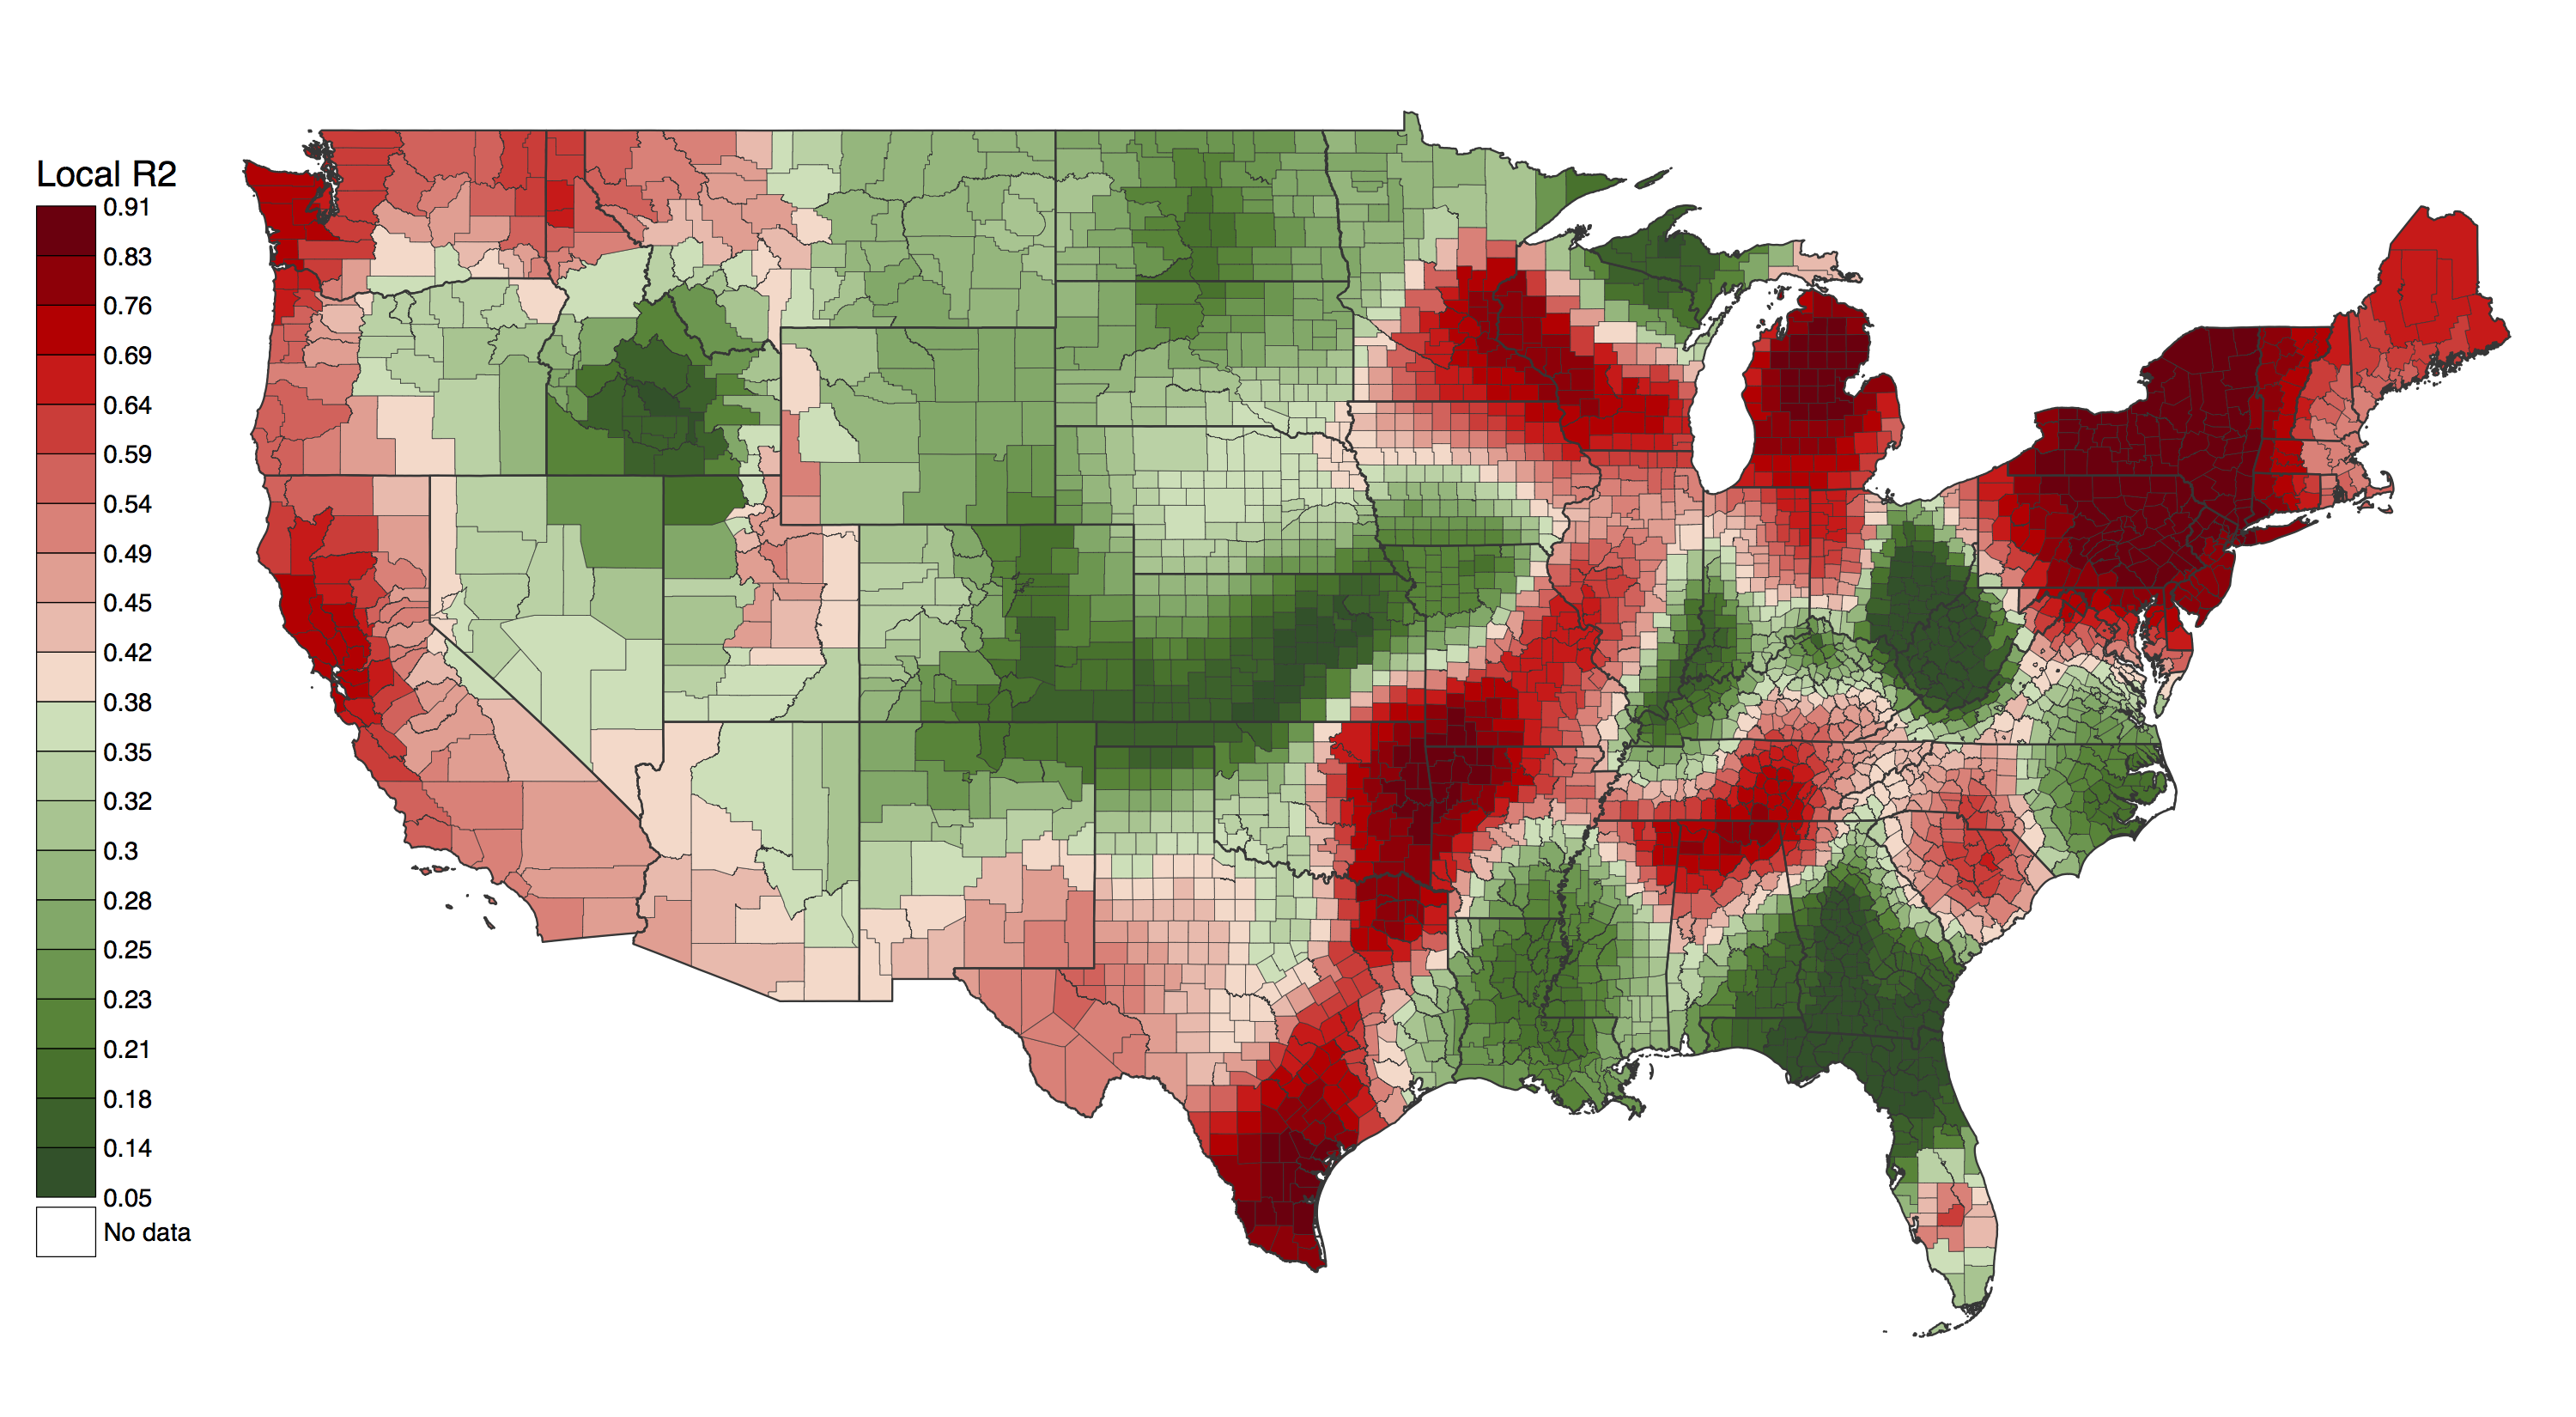
\includegraphics[width=0.49\linewidth]{Figures/EnergyPrice/gwr_allbest_LocalR2}
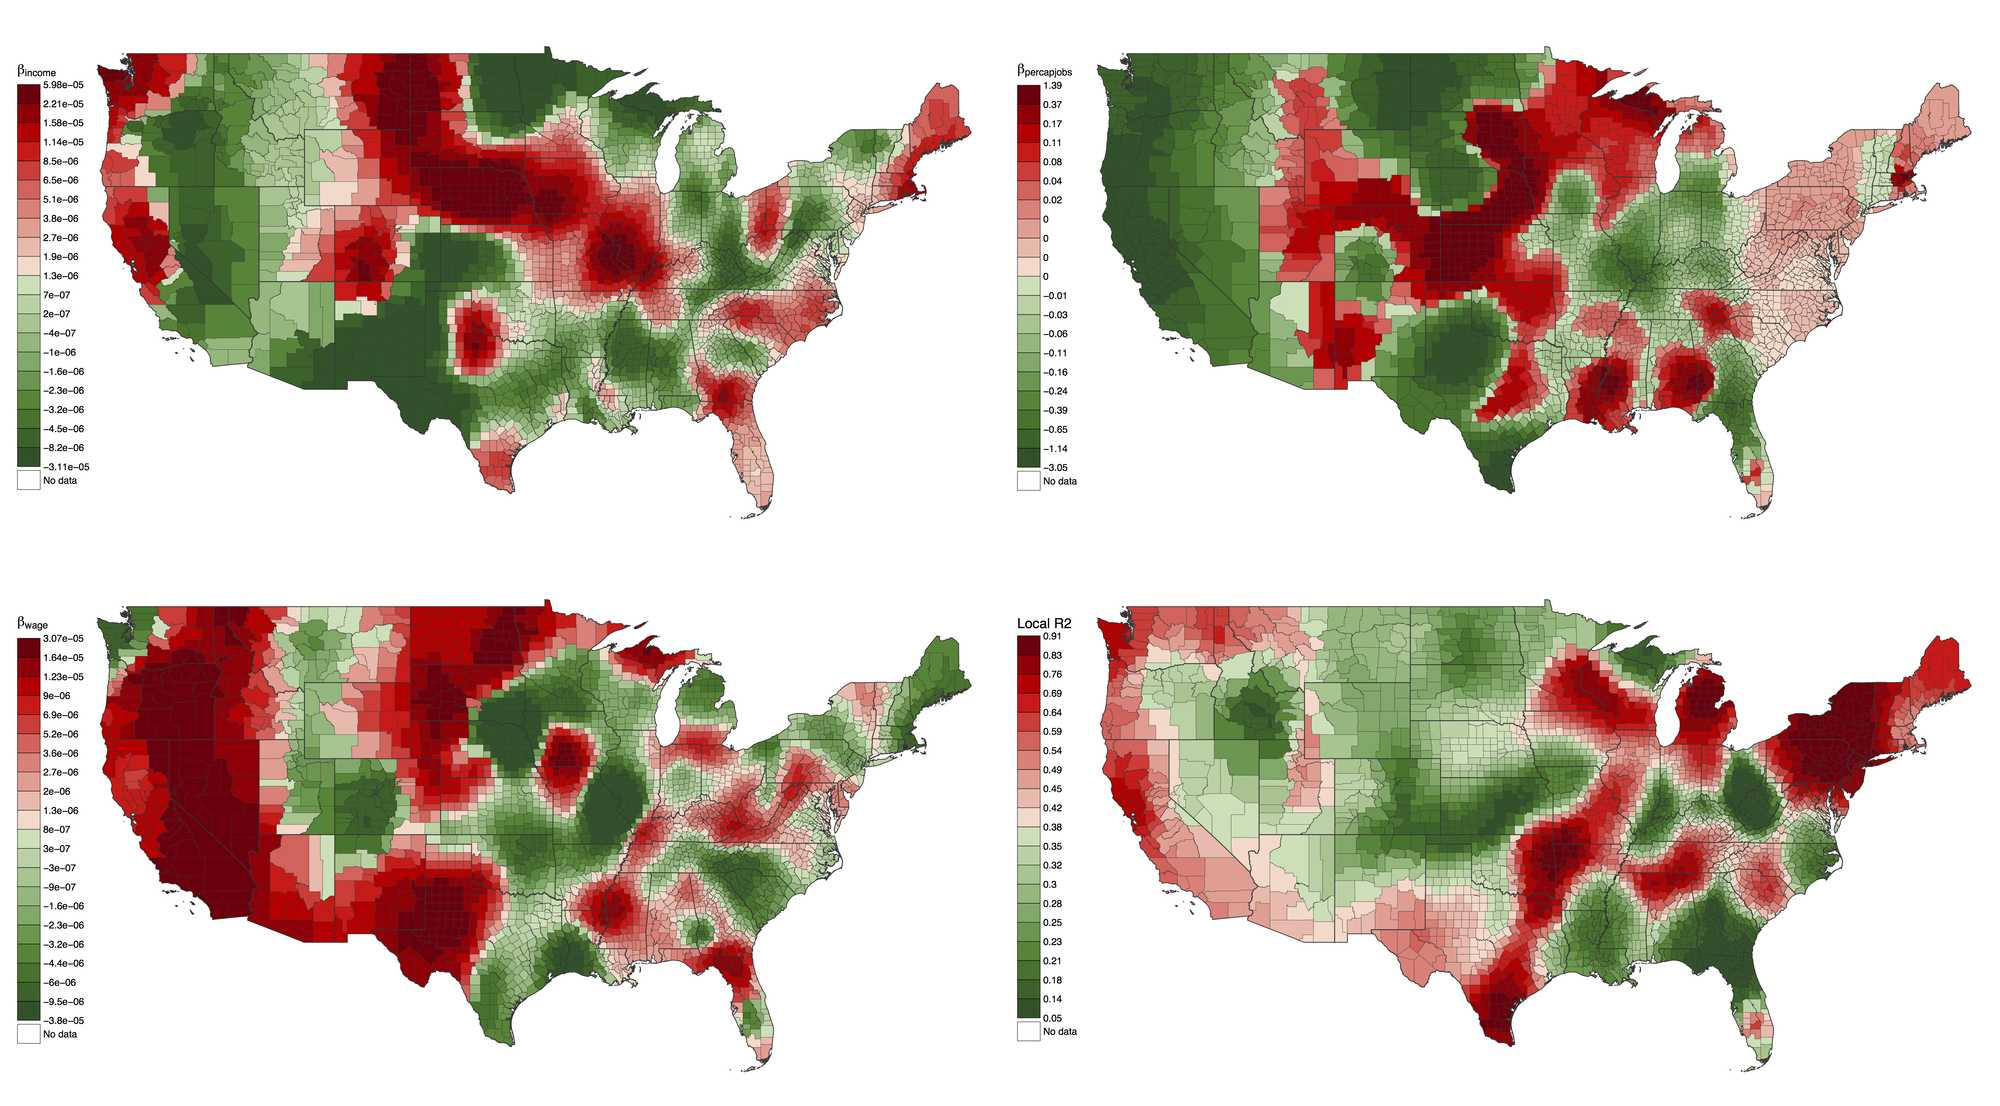
\includegraphics[width=\linewidth]{Figures/Final/8-2-2-fig-energyprice-gwr.jpg}
\caption[Results of GWR analyses][Résultats des analyses GWR]{\textbf{Results of GWR analyses.} For the best model in the sense of AICc, we map the spatial distribution of fitted coefficient, in order from left to right and top to bottom, $\beta_{income}$, $\beta_{percapjobs}$, $\beta_{wage}$, and finally the local r-squared values.\label{fig:energyprice:gwr}}{\textbf{Résultats des analyses GWR.} Pour le meilleur modèle au sens de l'AICc, les cartes donnent la distribution spatiale des coefficients estimés, dans l'ordre de gauche à droite et de haut en bas, $\beta_{income}$, $\beta_{percapjobs}$, $\beta_{wage}$, et finalement les valeurs du R2 local.\label{fig:energyprice:gwr}}
\end{figure}
%%%%%%%%%%%%%%%



\subsubsection{Multi-level Regression}{Régressions multi-niveaux}


\bpar{
Since our initial database enables to look at the level of variable $x_{i,s,c,t}$, the fuel price in day $t$, in gas station $i$, in state $s$ and in county $c$, we start by running high dimensional fixed effect regressions following the model:
}{
Comme notre base initiale permet de regarder au niveau des variables $x_{i,s,c,t}$, le prix du carburant au jour $t$, dans la station $i$, dans l'Etat $s$ et dans le Conté $c$, nous commençons par estimer des régressions à effets fixes en grande dimension, suivant les modèles :
}


\begin{eqnarray}
x_{i,s,c,t} &=& \beta_s + \varepsilon_{i,s,c,t} \\
x_{i,s,c,t} &=& \beta_c + \varepsilon_{i,s,c,t} \\
x_{i,s,c,t} &=& \beta_i + \varepsilon_{i,s,c,t}
\end{eqnarray}


\bpar{
Where $\varepsilon_{i,s,c,t}$ contains an idiosyncratic error and a day fixed effect. This first analysis confirm that most of the variance can be explained by a state fixed effect and that integrating more accurate levels has only small effect on the fit of our model as measured by the R-squared.
}{
Où $\varepsilon_{i,s,c,t}$ contient une erreur idiosyncrasique\footnote{C'est à dire étant propre à chaque individu.} et un effet fixe jour Cette première analyse confirme que la majorité de la variance peut être expliquée par un effet fixe au niveau de l'État et que d'intégrer des niveaux plus fins a un effet négligeable sur la performance du modèle mesurée par le R2.
}


\bpar{
We now turn to a different analysis, aiming at capturing the explanatory variables that account for spatial price variation of fuel. We consider the following linear model:
}{
Nous nous tournons à présent vers une analyse différente, visant à capturer les variables explicatives qui rendent compte des variations spatiales du carburant. Nous considérons le modèle linéaire suivant :
}


\begin{equation}
\label{eq:reg}
log(x_{i}) = \beta_0 + X_{i}\beta_1 + \beta_{s(i)} + \varepsilon_{i},
\end{equation}

\bpar{
where $x_{i}$ denotes average measured fuel price in county $i$ aggregated across all days, $X_{i}$ is a set of county specific variables and $s(i)$ is the state to which the county belongs so that $\beta_{s(i)}$ capture all state specific variation. Finally $\varepsilon_{i}$ is an error term satisfying $Cov(\varepsilon_{i}, \varepsilon_{j}) = 0$ if $s(i) \neq s(j)$. This clustering of standard error at the state level is motivated by finding of the previous section, showing that spatial autocorrelation of fuel price at the state level is still potentially strong. This specification aims at capturing the effect of various socio-economic variable at the county level after a state fixed effect has been removed.
}{
où $x_{i}$ dénote le prix moyen mesuré du carburant dans le Conté $i$ agrégé sur l'ensemble des jours, $X_{i}$ est un ensemble de variables spécifiques au Conté et $s(i)$ est l'état dans lequel se trouve le Conté de telle façon que $\beta_{s(i)}$ capture toute la variation spécifique aux Etats. Enfin $\varepsilon_{i}$ est un terme d'erreur satisfaisant $Cov(\varepsilon_{i}, \varepsilon_{j}) = 0$ si $s(i) \neq s(j)$. ce regroupement de l'erreur standard au niveau de l'état est motivé par les résultats de la partie précédente, montrant que l'autocorrélation spatiale des prix du carburant au niveau de l'état est toujours potentiellement forte. Cette spécification vise à capturer les effets de variables socio-économiques variées au niveau du Conté après que l'effet fixe Etat aie été retiré.
}


\bpar{
We present our results in Table~\ref{tab:reg}. Column (1) shows that regressing the log of price on a state fixed-effect is already enough to explain 74\% of the variance. This is mostly due to tax on fuel which are set at the state level in the US. In fact, when we regress the log of oil price on the level of state tax, we find a R-squared of 0.33\%. The remaining explanatory variables show that dense urban counties have higher fuel price, but this price decreases with population. This result seems sensible, desert areas have on average higher oil price. Fuel price increases with total income, decreases with poverty and decrease with the extent to which a county has voted for a Republican candidate. This last finding suggests a circular link: counties that use car the most tend to vote to politician that promote pro car policies. Adding these explanatory variables slightly increase the R-squared, suggesting that even after having removed a state fixed-effect, the price of fuel can be explained by local socio-economic features.	
}{
Les résultats sont présentés en Table~\ref{tab:energyprice:reg}. La première colonne montre que la regression du logarithme des prix sur un effet fixe Etat est déjà suffisant pour expliquer 74\% de la variance. Cela est majoritairement du aux taxes sur les carburants qui sont fixées au niveau de l'Etat aux Etats-Unis. En fait, une régression du log-prix sur le niveau de taxe donne un R-squared de 0.33\%. Les variables explicatives restantes montrent que les Contés urbains denses ont des prix plus élevés, mais que le prix décroit avec la population. Ce résultat paraît raisonnable, les zones désertiques ayant en moyenne des prix plus hauts. Les prix augmentent avec le revenu total, décroissent avec le niveau de pauvreté et décroisse avec le niveau de vote pour un candidat républicain. Ce dernier point suggère un lien circulaire : les Contés qui utilisent beaucoup la voiture auront tendance à voter pour un politicien qui promouvra des politiques favorable à son usage. L'ajout de ces variables explicatives augmente légèrement le R-squared, ce qui suggère que même après avoir enlevé l'effet fixe Etat, la prix du carburant peut être expliqué par des caractéristiques socio-économiques locales.
}



%%%%%%%%%%%%%%%
\begin{table}[htbp]
\vspace{-0.1cm}
\begin{center}
{
\begin{threeparttable}
\caption[Regressions at the county level][Régressions au niveau du comté]{Regressions at the county level\label{tab:energyprice:reg}}{\textbf{Régressions multi-niveau au niveau du comté.}\label{tab:energyprice:reg}}
\begin{tabular}{lccccc}
 \toprule
 \hline
 \cr

  & (1) & (2) & (3) & (4) & (5) \\ 
\cmidrule(r){2-6}
Density      &               &       0.016***&       0.016***&       0.016***&       0.015***\\
                    &               &     (0.002)   &     (0.001)   &     (0.001)   &     (0.001)   \\ \cr
Population (log)             &               &      -0.007***&      -0.040***&      -0.041***&      -0.039***\\                    &               &     (0.001)   &     (0.011)   &     (0.011)   &     (0.010)   \\ \cr
Total Income (log)            &               &               &       0.031***&       0.031***&       0.027***\\
                    &               &               &     (0.010)   &     (0.010)   &     (0.009)   \\ \cr
Unemployment        &               &               &       0.001   &       0.000   &       0.000   \\
                    &               &               &     (0.001)   &     (0.001)   &     (0.001)   \\ \cr
Poverty   &               &               &      -0.028** &      -0.030***&      -0.029** \\
                    &               &               &     (0.011)   &     (0.011)   &     (0.011)   \\ \cr
Percentage Black    &               &               &               &       0.000***&      -0.000   \\
                    &               &               &               &     (0.000)   &     (0.000)   \\ \cr
Vote GOP      &               &               &               &               &      -0.072***\\
                    &               &               &               &               &     (0.015)   \\ \cr 
\cmidrule{2-6}
R-squared           &       0.743   &       0.767   &       0.774   &       0.776   &       0.781   \\
N                   &        3,066   &        3,011   &        3,011   &        3,011   &        3,011   \\
\cr
\hline
\bottomrule
\end{tabular}
 \begin{tablenotes}
       \item \bpar{\protect\scriptsize{\textbf{Notes}: This table plots results from an Ordinary Least Square regression of model presented in equation (\ref{eq:reg}). Density is measured as the number of inhabitant by square miles and total income is given in dollars. Poverty is measured as the number of people below the poverty threshold per inhabitant. Percentage black is the percentage of black people living in the county and vote GOP is the share of people having voted for Donald Trump in the 2016 elections. Regression includes a state fixed effect. Robust standard errors clustered at the state level are reported in parenthesis. ***, ** and * respectively indicate 0.01, 0.05 and 0.1 levels of significance.}}{\protect\scriptsize{\textbf{Notes} : Cette table donne les résultats d'une régression des Moindres Carrés Ordinaire pour le modèle présenté en équation  (\ref{eq:reg}). La densité est mesurée comme le nombre d'habitants au mile-carré et le revenu total est donné en dollars. La pauvreté est mesurée comme le nombre de personnes sous le seuil de pauvreté par habitants. On étudie aussi l'influence du pourcentage de personnes noires et de la part de personnes ayant voté pour Donald Trump aux élections de 2016. La régression inclut un effet fixe Etat. Les erreurs standard robustes, agrégées au niveau de l'état, sont données entre parenthèses. ***, ** and * indiquent respectivement les niveau de significativité 0.01, 0.05 and 0.1.}}
    \end{tablenotes}
  \end{threeparttable}
}
\end{center}
\end{table}
%%%%%%%%%%%%%%%



%%%%%%%%%%%%%%%%%%%%%%
\subsection{Discussion}{Discussion} \label{sec:discuss}
%%%%%%%%%%%%%%%%%%%%%%

\subsubsection{On the complementarity of Econometric and Spatial Analysis methods}{Sur la complémentarité des méthodes économétriques et des méthodes d'analyse spatiale}

\bpar{
One important aspect of our contribution is methodological. We show that to explore a new panel dataset, geographers and economists have different approach, leading to similar generic conclusion but with different path. Some studies have already combined GWR and multi-level regressions (\cite{chen2012using}), or compared them in terms of model fit or robustness (\cite{lee2009determinants}). We take here a multi-disciplinary point of view and combines approaches answering to different questions, GWR aiming at finding precise explicative variables and to measure the extent of spatial correlation, whereas econometric models explain with more accuracy the effect of factors at different levels (state, county) but take these geographical characteristics as exogenous. We claim that both are necessary to understand all dimensions of the studied phenomenon.
}{
Un aspect important de cette contribution est méthodologique. Nous montrons que pour explorer un nouveau panel de données, les géographes et les économistes prennent des approches différentes, menant à des conclusions génériques similaires par des chemins différents. Des études ont déjà combiné les GWR et les régressions multi-niveau (\cite{chen2012using}), ou les ont comparées en terme de performance de modèle ou de robustesse (\cite{lee2009determinants}). Nous prenons ici un point de vue multi-disciplinaire et combinons des approches répondant à des questions différentes, GWR ayant pour but de trouver des variables explicatives précises et de mesurer le role de l'auto-corrélation spatiale, tandis que les modèles économétriques expliquent plus précisément les effets des différents facteurs à plusieurs niveaux (Etat, Conté) mais prennent ces caractéristiques géographiques comme exogènes. Nous postulons que les deux sont nécessaires pour comprendre toutes les dimensions du phénomène étudié.
}


\subsubsection{Designing localized car-regulation policies}{Proposition de politiques de régulation localisées}

\bpar{
Another application of such analysis is to help better designing car-regulation policies. Environmental and health issues nowadays require a reasoned use of cars, in cities with the problem air pollution but also overall to reduce carbon emissions. \cite{fullerton2002can} showed that a taxation of fuel and cars can be equivalent to a taxation on emissions. \cite{brand2013accelerating} highlight the role of incentives for the transition towards a low carbon transportation. However, such measures can't be uniform across states or even counties for obvious reasons of territorial equity: areas with different socio-economic characteristics or with different amenities shall contribute regarding their capabilities and preferences. Knowing local prices dynamics and their drivers, in which our study is a preliminary step, may be a path to localized policies taking into account the socio-economic configuration and include an equity criterion.
}{
Une autre application de ce type d'analyse est d'aider à une meilleure conception de politiques de régulation de la voiture. Les problèmes environnementaux et de santé requièrent de nos jours un usage raisonné de celle-ci, dans les villes avec le problème de la pollution atmosphérique, mais aussi globalement pour réduire les emissions de CO\textsubscript{2}. \cite{fullerton2002can} montre qu'une taxation des carburants et des voitures peut être équivalente à une taxation des emissions. \cite{brand2013accelerating} souligne le rôle des incitations pour une transition vers des transports décarbonés. Cependant, de telles mesures ne peuvent pas être uniformes d'un Etat à l'autre ou même entre les Contés, pour des raisons évidentes d'équité territoriale : des zones avec des caractéristiques socio-économiques différentes ou avec différentes aménités doivent contribuer selon leur possibilité et préférences. La connaissance des dynamiques locales des prix et leur déterminants, ce en quoi notre étude est une étape préliminaire, peut être une voie vers des régulations localisées prenant en compte la configuration socio-économique et inclure un critère d'équité.
}


%%%%%%%%%%%%%%%%%%%%%%
\subsubsection{Conclusion}{Conclusion}


\bpar{
We have described a first exploratory study of US fuel prices in space and time, using a new database at the gas station level spanning two months. We our first result is to show the high spatial heterogeneity of price processes, using interactive data exploration and auto-correlation analyses. We proceed with two complementary studies of potential drivers: GWR unveils spatial structures and geographical particularities, and yields a characteristic scale of processes around 75km; multi-level regressions show that even though most of the variation can be explained by state level characteristics, and mostly by the level of the tax on fuel that is set by the state, there are still socio-economic specificities at the county level that can explain spatial variation of fuel price.
}{
Nous avons décrit une première étude exploratoire des prix des carburants aux US dans le temps et l'espace, utilisant une nouvelle base de données au niveau de la station s'étendant sur deux mois. Notre premier résultat est de montrer la grande hétérogénéité spatiale des processus de prix, par une exploration interactive des données et des analyses d'auto-corrélation. Nous procédons à deux études complémentaires des déterminants potentiels : GWR révèle des structures spatiales et des particularités géographiques, and fournit une échelle caractéristique des processus autour de 75km ; les régressions multi-niveaux montrent que même si la majorité des variations sont expliquées par les caractéristiques des Etats, et majoritairement par le niveau de taxation fixé par l'Etat, il existe toujours des spécificités socio-économiques au niveau du Conté qui peuvent expliquer la variation spatiale des prix du carburant.
}



%%%%%%%%%%%%%%%%%%%%%%
\subsubsection{Perspective}{Mise en perspective}



\bpar{}{
Dans la perspective de notre problématique générale, cette deuxième ouverture empirique est ainsi pertinente pour différentes raisons : (i) la distribution spatiale des prix est un objet d'étude à la croisée des territoires et des réseaux, puisque les marchés locaux sont intimement liés aux caractéristiques territoriales, mais également déterminés par les propriété du réseau routier (par exemple accessibilité) et par ses motifs d'utilisation ; (ii) les deux échelles endogènes identifiées correspondent à nos échelles mesoscopique et macroscopique, confirmant par une autre approche la nécessité de prendre bien les deux en compte ; (iii) la mise en évidence de la superposition d'un processus de gouvernance à des processus géographiques locaux rejoint notre dernier développement sur la prise en compte de la gouvernance dans les modèles, puisque cette complexité est effectivement observée empiriquement ici.
}




\stars










